\documentclass[12pt]{article}
\usepackage[letterpaper, portrait, margin=1in]{geometry}
\usepackage{amsmath, amsthm, amssymb, mathrsfs}

\usepackage{graphicx}
\graphicspath{{/Users/darshanpatel/Desktop/LaTex Notes/CS220/}}

\usepackage{fancyhdr}
\pagestyle{fancy}
\fancyhf{}
\lhead{Darshan Patel}
\rhead{CS220: Discrete Structures}
\renewcommand{\footrulewidth}{0.4pt}
\cfoot{\thepage}

\begin{document}

\theoremstyle{definition}
\newtheorem{alg}{Algorithm}[section]
\newtheorem{theorem}{Theorem}[section]
\newtheorem{definition}{Definition}[section]
\newtheorem{example}{Example}[section]


\title{CS220: Discrete Structures}
\author{Darshan Patel}
\date{Spring 2017}
\maketitle

\tableofcontents
 \newpage
 
\section{Algoritms}
\subsection{Algorithms} 
\begin{definition} Algorithm: a finite sequence of precise instructions for performing a computation or for solving a problem \end{definition}
\begin{alg} Finding the Maximum Value in a Sequence of Integers: 
\begin{enumerate}
\item Set the temporary maximum equal to the first integer in the sequence 
\item Compare the next integer in the sequence to the temporary maximum, and if it is larger than the temporary maximum, set the temporary maximum equal to this integer 
\item Repeat the previous step if there are more integers in the sequence 
\item Stop when there are no integers left in the sequence \end{enumerate} 
The temporary maximum at this point is the largest integer in the sequence. \\~\\
procedure \textit{linear search}($x$:integer, $a_1, a_2, \dots, a_n$: distinct integers) \\ $i := 1$ \\ while($i \leq n$ and $x \neq a_i$) \\ \indent $i := i + 1$ \\ if $i \leq n$ then location $:= i$ \\ else location $:= 0$ \\ return location\{location is the subscript of the term that equals $x$, or is 0 if $x$ is not found\} \end{alg}
\begin{definition} Binary Search Algorithm: proceeds by comparing the element to be located to the middle term of the list; the list is then split into two smaller sublists of the same size, or where one of these smaller lists have one fewer than the other; the search continues by restricting the search to the appropriate sublist based on the comparison of the element to be located and the middle term \end{definition} 
\begin{alg} Binary Search Algorithm: \\ 
procedure \textit{binary search}($x$: integer, $a_1, a_2, \dots, a_n$: increasing integers) \\ $i := 1$\{$i$ is left endpoint of search interval\} \\ $j := n$\{$j$ is right endpoint of search interval\} \\ while $i < j$ \\ \indent $m := \lfloor (i + j)/2 \rfloor$ \\ \indent if $x > a_m$ then $i := m + 1$ \\ \indent else $j := m$ \\ if $x = a_i$ then location := $i$ \\ else location := 0 \\ return location\{location is the subscript $i$ of the term $a_i$ equal to $x$, or 0 if $x$ is not found\} \end{alg}
\begin{definition} Sorting: putting elements into a list in which the elements are in increasing order \end{definition} 
\begin{definition} Bubble Sort: puts a list into increasing order by successively comparing adjacent elements, interchanging them if they are in the wrong order \end{definition} 
\begin{alg} Bubble Sort: \\ procedure \textit{bubblesort}($a_1,\dots, a_n$: real numbers with $n \geq 2$) \\ for $i := 1$ to $n - 1$ \\ \indent for $j := 1$ to $n - i$ \\ \indent \indent if $a_j > a_{j + 1}$ then interchange $a_j$ and $a_{j + 1}$ \\ $\{a_1, \dots, a_n\}$ is in increasing order \end{alg}
\begin{definition} Insertion Sort: beginning with the second element, compare it with the first element and insert it before the first element if it does not exceed the first element and after the first element if it exceeds the first element; the third element is then compared with the first element, and if it is larger than the first element, it is compared with the second element; it is inserted into the correct positions when the last element is compared \end{definition} 
\begin{alg} Insertion Sort: \\
procedure \textit{insertion sort}($a_1, a_2, \dots, a_n$: real numbers with $n \geq 2$) \\ for $j := 2$ to $n$ \\ \indent $i := 1$ \\ \indent while $a_j > a_i$ \\ \indent \indent $i := i + 1$ \\ \indent $m := a_j$ \\ \indent for $k := 0$ to $j - i - 1$ \\ \indent \indent $a_{j - k} := a_{j - k - 1}$ \\ \indent $a_i := m$ \\ $\{a_1, \dots, a_n\}$ is in increasing order \end{alg}

\subsection{The Growth of Functions}
\begin{definition} Big-$O$ Notation: can estimate the growth of a function without worrying about constant multipliers or smaller order terms; do not have to worry about the hardware and software used to implement an algorithm \end{definition} 
\begin{definition} Let $f$ and $g$ be functions from the set of integers or the set of real numbers to the set of real numbers. We say that $f(x)$ is $O(g(x))$ if there are constants $C$ and $k$ such that $$|f(x)| \leq C|g(x)|$$ whenever $x > k$. This is read as ``$f(x)$ is big-oh of $g(x)$.'' \end{definition} 
\begin{definition} Witnesses: the constants $C$ and $k$ in the definition of big-$O$ \end{definition} 
To establish that $f(x)$ is $O(g(x))$ we need only one pair of witnesses to this relationship; that is, to show that $f(x)$ is $O(g(x))$, we need to find only one pair of $C$ and $k$, the witnesses, such that $|f(x)| \leq C|g(x)|$ whenever $x > k$. 
\begin{example} Show that $f(x) = x^2 + 2x + 1$ is $O(x^2)$. \\ 
When $x > 1$, it follows that $x < x^2$ and $1 < x^2$. Thus $$0 \leq x^2 + 2x + 1 \leq x^2 + 2x^2 + x^2 = 4x^2$$ whenever $x > 1$. Consequently, $C = 4$ and $k = 1$ as witnesses to show that $f(x)$ is $O(x^2)$. That is, $f(x) = x^2 + 2x + 1 \leq 4x2$ whenever $x > 1$. \\~\\
Alternatively, when $x > 2$, we have $2x \leq x^2$ and $1 < x^2$. Thus $$ 0 \leq x^2 + 2x + 1 \leq x^2 + x^2 + x^2 = 3x^2$$ It follows that $C = 3$ and $k = 2$ are also witnesses to the relation $f(x) = O(x^2)$. \\~\\
Note: In the relationship $f(x)$ is $O(x^2)$, $x^2$ can be replaced by any function with larger values than $x^2$. For example, $f(x)$ is $O(x^3)$, $f(x)$ is $O(x^2 + x + 7)$, so forth. It is also true that $x^2$ is $O(x^2 + 2x + 1)$ because $x^2 < x^2 + 2x + 1$ whenever $x > 1$. This means that $C = 1$ and $k = 1$ are witnesses to the relationship $x^2$ is $O(x^2 + 2x + 1)$  \end{example}
\begin{definition} Same Order: exhibited by two functions $f(x)$ and $g(x)$ where $f(x)$ is $O(g(x))$ and $g(x)$ is $O(f(x))$ \end{definition} 
When $f(x)$ is $O(g(x))$, and $h(x)$ is a function that has larger absolute values than $g(x)$ does for sufficiently large values of $x$, it follows that $f(x)$ is $O(h(x))$. The function $g(x)$ in the relationship $f(x)$ is $O(g(x))$ can be replaced by a function with larger absolute values. \\~\\
Note: When big-$O$ notation is used, the function $g$ in the relationship $f(x)$ is $O(g(x))$ is chosen to be as small as possible. 
\begin{example} Show that $7x^2$ is $O(x^3)$. \\ 
When $x > 7$, we have $7x^2 < x^3$. Consequently, we can take $C = 1$ and $k = 7$ as witnesses to establish the relationship $7x^2$ is $O(x^3)$. Alternatively, when $x > 1$, we have $7x^2 < 7x^3$, so that $C = 7$ and $k = 1$ are also witnesses to the relationship $7x^2$ is $O(x^3)$. \end{example} 
\begin{example} Show that $n^2$ is not $O(n)$. \\ 
We must show that no pair of witnesses $C$ and $k$ exist such that $n^2 \leq Cn$ whenever $n > k$. \\Proof by contradiction: Suppose that there are constants $C$ and $k$ for which $n^2 \leq Cn$ whenever $n > k$. When $n > 0$, we can divide both sides by $n$ to obtain $n \leq C$. However, no matter what $C$ and $k$ are, the inequality $n \leq C$ cannot hold for all $n$ with $n > k$. Once we set a value of $k$, we see that when $n$ is larger than the maximum of $k$ and $C$, it is not true that $n \leq C$ even though $n > k$. This contradiction shows that $n^2$ is not $O(n)$. \end{example} 
\begin{example} Is it true that $x^3$ is $O(7x^2)$? \\ 
To determine whether $x^3$ is $O(7x^2)$, we need to determine whether witnesses $C$ and $k$ exist so that $x^3 \leq C(7x^2)$ whenever $x > k$. We will show that no such witnesses exist using a proof by contradiction \\ If $C$ and $k$ are witnesses, the inequality $x^3 \leq C(7x^2)$ holds for all $x > k$. Observe that the inequality is equivalent to $x \leq 7C$, which follows by dividing both sides by the positive quantity $x^2$. However, no matter what $C$ is, it is not the case that $x \leq 7C$ for all $x > k$ no matter what $k$ is, because $x$ can be made arbitrary large. It follows that no witnesses $C$ and $k$ exist for this proposed big-$O$ relationship. Hence, $x^3$ is not $O(7x^2)$. \end{example} 
\begin{theorem} Let $f(x) = a_nx^n + a_{n - 1}x^{n - 1} + \dots + a_1x + a_0$, where $a_0, a_1, \dots, a_{n - 1}, a_n$ are real numbers. Then $f(x)$ is $O(x^n)$. \end{theorem} 
\begin{example} How can big-$O$ notation be used to estimate the sum of the first $n$ positive integers? \\ 
Each integer in the sum of the first $n$ positive integers does not exceed $n$, thus it follows that $$1 + 2 + \dots + n \leq n + n + \dots + n = n^2$$
From this equality it follows that $1+ 2 + 3 + \dots + n$ is $O(n^2)$, taking $C = 1$ and $k = 1$ as witnesses \end{example} 
\begin{example} Give big-$O$ estimates for the factorial function and the logarithm of the factorial function, where the factorial function $f(n) = n!$ is defined by $n! = 1 \cdot 2 \cdot 3 \cdot \dots \cdot n$ whenever $n$ is a positive integer, and $0! = 1$. \\ A big-$O$ estimate for $n!$ can be obtained by noting that each term in the product does not exceed $n$. Hence $$ n! = 1 \cdot 2 \cdot 3 \cdot \dots \cdot n \leq n \cdot n \cdot n \cdot \dots \cdot n = n^n$$ This inequality shows that $n!$ is $O(n^n)$, taking $C = 1$ and $k = 1$ as witnesses. Taking logarithms of both sides of the inequality established for $n!$ shows $$ \log(n!) \leq \log(n^n) = n\log(n)$$ This implies that $\log(n!)$ is $O(n\log(n))$, again taking $C = 1$ and $k = 1$ as witnesses. \end{example}
\begin{example} Since $n < 2^n$, show that this inequality implies that $n$ is $O(2^n)$ and use this inequality to show that $\log(n)$ is $O(n)$. \\ 
Conclude that $n$ is $O(2^n)$ by taking $C = k = 1$ as witnesses. Because the logarithm function is increasing, take logarithms of base 2 on both sides of this inequality to show that $\log(n) < n$. It follows that $\log(n)$ is $O(n)$ with $C = k = 1$ as witnesses. \\~\\ If we have logarithms to a base $b$, where $b$ is different from 2, we still have $\log_b(n)$ is $O(n)$ because $$\log_b(n) = \frac{\log(n)}{\log(b)} \leq \frac{n}{\log(b)} $$ whenever $n$ is a positive integer. We take $C = \frac{1}{\log(b)}$ and $ k = 1$ as witnesses. \end{example} 
Note: If $d > c > 1$, then $n^c$ is $O(n^d)$, but $n^d$ is not $O(n^c)$. \\~\\ 
Note: Whenever $b > 1$ and $c$ and $d$ are positive, we have $(\log_b(n))^c$ is $O(n^d)$ but $n^d$ is not $(O(\log_b(n))^c)$. Every positive power of the logarithm of $n$ to the base $b$, where $b > 1$, is big-$O$ of every positive power of $n$, but the reverse relationship never holds. \\~\\ 
Note: Whenever $d$ is positive and $b > 1$, we have $n^d$ is $O(b^n)$ but $b^n$ is not $O(n^d)$. This tells us that every power of $n$ is big-$O$ of every exponential function of $n$ with a base that is greater than one, but the reverse relationship never holds. \\~\\ 
Note: Furthermore, we have when $c > b > 1$, $b^n$ is $O(c^n)$ but $c^n$ is not $O(b^n)$. This tells us that if we have two exponential functions with different bases greater than one, one of these functions is big-$O$ of the other if and only if its base is smaller or equal. 
\begin{theorem} Suppose that $f_1(x)$ is $O(g_1(x))$ and $f_2(x)$ is $O(g_2(x))$. Then $(f_1 + f_2)(x)$ is $O(\max(|g_1(x)|, |g_2(x)|))$. \end{theorem}
\begin{theorem} Suppose that $f_1(x)$ and $f_2(x)$ are both $O(g(x))$. Then $(f_1 + f_2)(x)$ is $O(g(x))$. \end{theorem} 
\begin{theorem} Suppose that $f_1(x)$ is $O(g_1(x))$ and $f_2(x)$ is $O(g_2(x))$. Then $(f_1f_2)(x)$ is $O(g_1(x)g_2(x))$. \end{theorem} 
\begin{example} Give a big-$O$ estimate for $f(n) = 3n\log(n!) + (n^2 + 3)\log(n)$, where $n$ is a positive integer. \\ First, the product $3n\log(n!)$ will be estimated. We know from earlier that $\log(n!)$ is $O(n\log(n))$. Using this estimate and the fact that $3n$ is $O(n)$, the estimate of this product is $O(n\log(n) \times n)$ or $O(n^2\log(n))$. Next, the product $(n^2 + 3)\log(n)$ will be estimated. Because $(n^2 + 3) < 2n^2$ when $n > 2$, it follows that $n^2 + 3$ is $O(n^2)$. Thus the estimate of this product is also $O(n^2\log(n))$. Since both $f_1$ and $f_2$ have the same $O(g(x))$, the sum of them show that $f(n)$ is $O(n^2\log(n))$. \end{example} 
\begin{example} Give a big-$O$ estimate for $f(x) = (x + 1)\log(x^2 + 1) + 3x^2$. \\ First, a big-$O$ estimate for $(x + 1)\log(x^2 + 1)$ will be found. Note that $(x + 1)$ is $O(x)$. Furthermore, $x^2 + 1 \leq 2x^2$ when $x > 1$. Hence $$ \log(x^2 + 1) \leq \log(2x^2) = \log(2) + \log(x^2) = \log(2) + 2\log(x) \leq 3\log(x) $$ if $x > 2$> This shows that $\log(x^2 + 1)$ is $O(\log(x))$. It follows tat $(x + 1)\log(x^2 + 1)$ is $O(x\log(x))$. Because $3x^2$ is $O(x^2)$, $f(x)$ is $O(\max(x\log(x), x^2))$. Because $x\log(x) < x^2$, for $x > 1$, it follows that $f(x)$ is $O(n^2)$. \end{example} 
\begin{definition} Big-$\Omega$ Notation: provides a lower bound for the size of $f(x)$ for large $x$ \end{definition} 
\begin{definition} Big-$\Theta$ Notation: provides both an upper and a lower bound on the size of a function $f(x)$, relative to a reference function $g(x)$ \end{definition} 
\begin{definition} Let $f$ and $g$ be functions from the set of integers or the set of real numbers to the set of real numbers. We say that $f(x)$ is $\Omega(g(x))$ if there are positive constants $C$ and $k$ such that $|f(x)| \geq C|g(x)|$ whenever $x > k$. This is read as ``$f(x)$ is big-Omega of $g(x)$.'' \end{definition} 
Note: $f(x)$ is $\Omega(g(x))$ if and only if $g(x)$ is $O(f(x))$. 
\begin{example} The function $f(x) = 8x^3 + 5x^2 + 7$ is $\Omega(g(x))$, where $g(x)$ is the function $g(x) = x^3$. This is easy to see because $f(x) = 8x^3 + 5x^2 + 7 \geq 8x^3$ for all positive real numbers $x$. This is equivalent to saying that $g(x) = x^3$ is $O(8x^3 + 5x^2 + 7)$, which can be established directly by turning the inequality around. \end{example} 
\begin{definition} Let $f$ and $g$ be functions from the set of integers or the set of real numbers to the set of real numbers. We say that $f(x)$ is $\Theta(g(x))$ if $f(x)$ is $O(g(x))$ and $f(x)$ is $\Omega(g(x))$. When $f(x)$ is $\Theta(g(x))$, we say that $f$ is big-Theta of $g(x)$, that $f(x)$ is of order $g(x)$, and that $f(x)$ and $g(x)$ are of the same order. \end{definition} 
Note: When $f(x)$ is $\Theta(g(x))$, it is also the case that $g(x)$ is $\Theta(f(x))$. Also, $f(x)$ is $\Theta(g(x))$ if and only if $f(x)$ is $O(g(x))$ and $g(x)$ is $O(f(x))$. Furthermore, note that $f(x)$ is $\Theta(g(x))$ if and only if there are real numbers $C_1$ and $C_2$ and a positive real number $k$ such that $$C_1|g(x)| \leq f(x) \leq C_2|g(x)| $$ whenever $x > k$. The existence of the constants $C_1$, $C_2$ and $k$ tells us that $f(x)$ is $\Omega(g(x))$ and that $f(x)$ is $O(g(x))$. 
\begin{example} Since the sum of the first $n$ positive integers if $O(n^2)$, is this sum of order $n$? \\ 
Let $f(n) = 1 + 2 + \dots + n$. We already know that $f(n)$ is $O(n^2)$ t. To show that $f(n)$ is of order $n^2$, we need to find a positive constant $C$ such that $f(n) > Cn^2$ for sufficiently large integers $n$. To obtain a lower bound for this sum, we can ignore the first half of the terms . Summing only the terms greater than $\Big\lceil \frac{n}{2} \Big\rceil$, we find that $$ \begin{aligned} 1 + 2 + \dots + n &\geq \Big\lceil \frac{n}{2} \Big\rceil + (\Big\lceil \frac{n}{2} \Big\rceil + 1) + \dots + n \\ &\geq \Big\lceil \frac{n}{2} \Big\rceil + \Big\lceil \frac{n}{2} \Big\rceil + \dots + \Big\lceil \frac{n}{2} \Big\rceil = (n - \Big\lceil \frac{n}{2} \Big\rceil + 1)\Big\lceil \frac{n}{2} \Big\rceil \\ &\geq (\frac{n}{2})(\frac{n}{2}) \\ &= \frac{n^2}{4} \end{aligned} $$ This shows that $f(n)$ is $\Omega(n^2)$. We conclude that $f(n)$ is of order $n^2$, or in symbols, $f(n)$ is $\Theta(n^2)$. \end{example} 
\begin{example} Show that $3x^2 + 8x\log(x)$ is $\Theta(x^2)$. \\ 
Because $0 \leq 8x\log(x) \leq 8x^2$, it follows that $3x^2 + 8x\log(x) \leq 11x^2$ for $x > 1$. Consequently, $3x^2 + 8x\log(x)$ is $O(x^2)$. Clearly, $x^2$ is $O(3x^2 + 8x\log(x))$. Consequently, $3x^2 + 8x\log(x)$ is $\Theta(x^2)$. \end{example} 
\begin{theorem} Let $f(x) = a_nx^n + a_{n - 1}x^{n - 1} + \dots + a_1x + a_0$, where $a_0, a_1, \dots, a_n$ are real numbers with $a_n \neq 0$. Then $f(x)$ is of order $x^n$. \end{theorem} 
\begin{example} The polynomials $3x^8 + 10x^7 + 221x^2 + 1444$, $x^{19} - 18x^4 - 10112$, and $-x^{99} + 40001x^{98} + 100003x$ are of orders $x^8$, $x^{19}$, and $x^{99}$, respectively. \end{example}

\begin{example} Find Big-$O$ of $f(n) = n\log(n^2 + 1) + n^2log(n)$. 
$$ \begin{aligned} \log(n^2 + 1) &\leq \log(n^2 + n^2)  \\ &= \log(2n^2) \\ &= \log(2) + \log(n^2) \\ &= \log(2) + 2\log(n) \\ &\leq \log(n) + 2\log(n) \\ &= 3\log(n) \end{aligned} $$  
$n\log(n^2 + 1)$ is $n\cdot 3\log(n)$ or $O(n\log(n))$. But $n^2\log(n)$ is larger than $n\log(n)$ thus $n\log(n^2 + 1) + n^2\log(n)$ is $O(n^2\log(n))$. \end{example}
\begin{example} Find Big-$O$ of $f(n) = n^{2^n} + n^{n^2} $. \\~\\
$2^n$ grows faster thus $O(2^{n^2})$. \end{example} 
\begin{example} Find $f(n)$ such that $f(n) = O(\log_{10}(n))$ and $f(n) = \Omega(\log_5(n))$.  
$$ f(n) = O(\log(n)) $$
Base does not matter. \end{example} 
\begin{example} Find a function $f(n)$ where $f(n) = \Omega(n!)$ and $f(n) = O(n^n)$.
$$f(n) = n!$$ \end{example} 
\begin{example} Find a function $f(n)$ where $f(n) = \Omega(n^n)$ and $f(n) = O(n!)$. \\~\\
This is not possible bc $n^n$ is larger than $n!$. Lower limit is bigger than upper limit. \end{example} 
\begin{example} Find a function $f(n)$ where $f(n) = \Omega(n^2)$ and $f(n) = O(n^2 + n)$.  
\\~\\Use $f(n) = n^2$ because $\Omega$ and $O$ are similar. \end{example} 
\begin{example} Find a function $f(n)$ where $f(n) = \Omega(3n^n)$ and $f(n) = O(15n!)$. \\~\\ Not possible. \end{example} 
\begin{example} Find a function $f(n)$ where $f(n) = \theta(n^2)$ and $f(n) = \Omega(n)$. $$ f(n) = n^2 $$ \end{example}

\subsection{Complexity of Algorithms}
\begin{definition} Time Complexity: an analysis of the time required to solve a problem of a particular size \end{definition} 
\begin{definition} Space Complexity: an analysis of the computer memory required to solve a problem \end{definition} 
The time complexity of an algorithm can be expressed in terms of the number of operations used by the algorithm when the input has a particular size. The operations used to measure time complexity an be the comparison of integers, the addition of integers, the multiplication of integers, the division of integers, or any other basic operation. 
\begin{example} Describe the time complexity for finding the maximum element in a finite set of integers. \\ To find the maximum element of a set with $n$ elements, listed in an arbitrary order, the temporary maximum is first set equal to the initial term in the list. Then, after a comparison $ i \leq n$ has been done to determine that the end of the list has not yet been reached, the temporary maximum and second term are compared, updating the temporary maximum to the value of the second term if it is larger. The procedure is continued, using two additional comparisons for each term of the list - one $ i \leq n$, to determine that the end of the list has not been reached and another max $< a_i$, to determine whether to update the temporary maximum. Because two comparisons are used for each of the second through the $n$th elements and one more comparison is used to exit the loop when $i = n + 1$, exactly $2(n + 1) + 1 = 2n - 1$ comparisons are used whenever this algorithm is applied. Hence, the algorithm for finding the maximum of a set of $n$ elements has time complexity $\Theta(n)$, measured in terms of the number of comparisons used. Note that for this algorithm, the number of comparisons is independent of particular input of $n$ numbers. \end{example} 

\begin{example} Describe the time complexity of the linear search algorithm. \\ The number of comparisons used will be taken as the measure of the time complexity. At each step of the loop in the algorithm, two comparisons are performed - one $i \leq n$, to see whether the end of the list has been reached and one $x \leq a_i$ , to compare the element $x$ with a term of the list. Finally, one more comparison $i \leq n$ is made outside the loop. Consequently, if $x = a_i$ , $2i + 1$ comparisons are used. The most comparisons, $2n + 2$, are required when the element is not in the list. In this case, $2n$ comparisons are used to determine that $x$ is not $a_i$, for $i = 1, 2, \dots, n$, an additional comparison is used to exit the loop, and one comparison is made outside the loop. So when $x$ is not in the list, a total of $2n + 2$ comparisons are used. Hence, a linear search requires $\Theta(n)$ comparisons in the worst case, because $2n + 2$ is $\Theta(n)$. \end{example}
\begin{definition} Worst-Case Analysis: a type of analysis that gives the largest number of operations needed to solve the given problem using the algorithm on put of specified size; tells how many operations an algorithm requires to guarantee that it will produce a solution \end{definition}

\begin{example} Describe the time complexity of the binary search algorithm in terms of the number of comparisons used (and ignoring the time required to compute $m = \lfloor (i + j)/2 \rfloor $ in each iteration of the loop in the algorithm). \\ 
For simplicity, assume there are $n = 2^k$ elements in the list $a_1, a_2,\dots, a_n$, where $k$ is a nonnegative integer. Note that $k = \log(n)$. (If $n$, the number of elements in the list, is not a power of 2, the list can be considered part of a larger list with $2^{k+1}$ elements, where $2^k < n < 2^{k+1}$. Here $2^{k+1}$ is the smallest power of 2 larger than $n$.) At each stage of the algorithm, $i$ and $j$, the locations of the first term and the last term of the restricted list at that stage, are compared to see whether the restricted list has more than one term. If $i < j$ , a comparison is done to determine whether $x$ is greater than the middle term of the restricted list. At the first stage the search is restricted to a list with $2^{k - 1}$ terms. So far, two comparisons have been used. This procedure is continued, using two comparisons at each stage to restrict the search to a list with half as many terms. In other words, two comparisons are used at the first stage of the algorithm when the list has $2^k$ elements, two more when the search has been reduced to a list with $2^{k - 1}$ elements, two more when the search has been reduced to a list with $2^{k - 2}$ elements, and so on, until two comparisons are used when the search has been reduced to a list with $2^1 = 2$ elements. Finally, when one term is left in the list, one comparison tells us that there are no additional terms left, and one more comparison is used to determine if this term is $x$. Hence, at most $2k + 2 = 2\log(n) + 2$ comparisons are required to perform a binary search when the list being searched has $2^k$ elements. (If $n$ is not a power of 2, the original list is expanded to a list with $2^{k + 1}$ terms, where $k = \lfloor \log(n)\rfloor$, and the search requires at most $2\lceil \log(n)\rceil + 2$ comparisons.) It follows that in the worst case, binary search requires $O(\log(n))$ comparisons. Note that in the worst case, $2\log(n) + 2$ comparisons are used by the binary search. Hence, the binary search uses $\Theta(\log(n))$ comparisons in the worst case, because $2\log(n) + 2 = \Theta(\log(n))$. From this analysis it follows that in the worst case, the binary search algorithm is more efficient than the linear search algorithm, because the linear search algorithm has $\Theta(n)$ worst-case time complexity.\end{example}
\begin{definition} Average-Case Analysis: a type of analysis where the average number of operations used to solve the problem over all possible inputs of a given size is found \end{definition} 
\begin{example} Describe the average-case performance of the linear search algorithm in terms of the average number of comparisons used, assuming that the integer $x$ is in the list and it is equally likely that $x$ is in any position. \\ 
By hypothesis, the integer $x$ is one of the integers $a_1, a_2, \dots, a_n$ in the list. If $x$ is the first term $a_1$ of the list, three comparisons are needed, one $i \leq n$ to determine whether the end of the list has been reached, one $x \neq a_i$ to compare $x$ and the first term, and one $i \leq n$ outside the loop. If $x$ is the second term $a_2$ of the list, two more comparisons are needed, so that a total of five comparisons are used. In general, if $x$ is the $i$th term of the list $a_i$, two comparisons will be used at each of the $t$ steps of the loop, and one outside the loop, so that a total of $2i + 1$ comparisons are needed. Hence the average number of comparisons used equals $$\frac{3 + 5 + 7 + \dots + (2n + 1)}{n} = \frac{2(1 + 2 + 3 + \dots + n) + n}{n} $$ By simplification, the average number of comparisons used by the linear search algorithm is: $$  \frac{2[n(n + 1)/2]}{n} + 1 = n + 2 $$ which is $\Theta(n)$. \end{example} 
\begin{example} What is the worst-case complexity of the bubble sort in terms of the number of comparisons made? \\ The bubble sort sorts a list by performing a sequence of passes through the list. During each pass the bubble sort successively compares adjacent elements, interchanging them if necessary. When the $i$th pass begins, the $i - 1$ largest elements are guaranteed to be in the correct positions. During this pass, $n - i$ comparisons are used. Consequently, the total number of comparisons used by the bubble sort to order a list of $n$ elements is: $$(n - 1) + (n - 2) + \dots + 2 + 1 = \frac{(n - 1)n}{2} $$ Note that the bubble sort always uses this many comparisons, because it continues even if the list becomes completely sorted at some intermediate step. Consequently, the bubble sort uses $(n - 1)n/2$ comparisons, so it has $\Theta(n^2)$ worst-case complexity in terms of the number of comparisons used. \end{example} 
\begin{example} What is the worst-case complexity of the insertion sort in terms of the comparisons made? \\ The insertion sort inserts the $j$th element into the correct position among the first $j - 1$ elements that have already bene put into the correct order. It does this by using a linear search technique, successively comparing the $j$th element with successive terms until a term that is greater than or equal to it is found or it compares $a_j$ with itself and stops because $a_j$ is not less than itself. Consequently, in the worst case, $j$ comparisons are required to insert the $j$th element into the correct position. Therefore, the total number of comparisons used by the insertion sort to sort a list of $n$ elements is: $$ 2 + 3 + \dots + n = \frac{n(n + 1)}{2} - 1$$ Note that the first term, 1, is missing in this sum. Note that the insertion sort may use considerably fewer comparisons if the smaller elements started out at the end of the list. Thus, the insertion sort has worst-case complexity of $\Theta(n^2)$. \end{example} 
Suppose that $C = [c_{ij}]$ is the $m \times n$ matrix that is the product of the $m \times k$ matrix $A = [a_{ij}]$ and the $k \times n$ matrix $B = [b_{ij}]$. 
\begin{alg} Matrix Multiplication: 
procedure \textit{matrix multiplication}($A, B$: matrices) \\
for $i := 1$ to $m$ \\
\indent for $j := 1$ to $n$ \\
\indent \indent $c_{ij} := 0$ \\
\indent \indent for $q := 1$ to $k$ \\ 
\indent \indent \indent $c_{ij} := c_{ij} + a_{iq}b_{qj}$ \\
return $C$ $\{C = [c_{ij}]$ is the product of $A$ and $B\}$ \end{alg} 
\begin{example} How many additions of integers and multiplication of integers are used to multiply two $n \times n$ matrices with integer entries? \\ There are $n^2$ entries in the product of $A$ and $B$. To find each entry requires a total of $n$ multiplications and $n - 1$ additions. Hence, a total of $n^3$ multiplications and $n^2(n - 1)$ additions are used. Thus it is $O(n^3)$. \end{example} 
Complexity of Algorithms $$\begin{tabular}{|c|c|} \hline 
Complexity & Terminology \\ \hline
$\Theta(1)$ & Constant complexity \\ \hline
$\Theta(\log(n))$ & Logarithmic complexity \\ \hline
$\Theta(n)$ & Linear complexity \\ \hline
$\Theta(n\log(n))$ & Linearithmic complexity \\ \hline
$\Theta(n^b)$ & Polynomial complexity \\ \hline
$\Theta(b^n) \text{, where } b > 1$ & Exponential complexity \\ \hline
$\Theta(n!)$ & Factorial complexity \\ \hline \end{tabular} $$ 


\section{Number Theory and Cryptography}
\subsection{Divisibility and Modular Arithmetic} 
\begin{definition} If $a$ and $b$ are integers, with $a \neq 0$, we say that $a$ divides $b$ if there is an integer $c$ such that $b = ac$, or equivalently, if $\frac{b}{a}$ is an integer. When $a$ divides $b$, we say that $a$ is a factor or divisor of $b$, and that $b$ is a multiple of $a$. The notation $a \mid b$ denotes that $a$ divides $b$. The notation $a \nmid b$ denotes that $a$ does not divide $b$. \end{definition} 
\begin{example} Let $n$ and $d$ be positive integers. How many positive integers not exceeding $n$ are divisible by $d$? \\ The positive integers divisible by $d$ are all the integers of the form $dk$, where $k$ is a positive integer. Hence, the number of positive integers divisible by $d$ that do not exceed $n$ equals the number of integers $k$ with $0 < dk \leq n$, or with $0 < k \leq n/d$. Therefore there are $\lfloor n/d \rfloor$ positive integers not exceeding $n$ that are divisible by $d$. \end{example} 
\begin{theorem} Let $a$, $b$, and $c$ be integers, where $a \neq 0$. Then \begin{itemize} 
\item if $a \mid b$ and $b \mid c$, then $a \mid (b + c)$ 
\item if $a \mid b$, then $a \mid bc$ for all integers $c$ 
\item if $a \mid b$ and $b \mid c$, then $a \mid c$ \end{itemize} \end{theorem} 
\begin{theorem} If $a$, $b$ and $c$ are integers, where $a \neq 0$, such that $a \mid b$ and $a \mid c$, then $a \mid mb + nc $ whenever $m$ and $n$ are integers. \end{theorem} 
\begin{theorem} Let $a$ be an integer and $d$ a positive integer. Then there are unique integers $q$ are $r$, with $ 0 \leq r < d$, such that $a = dq + r$. \end{theorem} 
\begin{definition} In the equality above, $d$ is called the divisor, $a$ is called the dividend, $q$ is called the quotient and $r$ is called the remainder. This notation is used to express the quotient and remainder: $$q = a \text{ div } d$$ $$r = a \text{ mod } d $$ \end{definition} 
\begin{example} What are the quotient and remainder when 101 is divided by 11? \\ We have $$101 = 11 \cdot 9 + 2$$ Hence, the quotient when 101 is divided by 11 is 9 = 101 div 11, and the remainder is 2 = 101 mod 11. \end{example} 
\begin{example} What are the quotient and remainder when -11 is divided by 3? \\ We have $$ -11 = 3(-4) + 1$$ Hence, the quotient when -11 is divided by 3 is -4 = -11 div 3 and the remainder is 1 = -11 mod 3. Note that the remainder cannot be negative. Consequently, the remainder is not -2, even though $-11 = 3(-3) - 2$ because $r = -2$ does not satisfy $0 \leq r < 3$. \end{example} 
\begin{definition} If $a$ and $b$ are integers and $m$ is a positive integer, then $a$ is congruent to $b$ modulo $m$ if $m$ divides $a - b$. We use the notation $a \equiv b \mod m$ to indicate that $a$ is congruent to $b$ modulo $m$. We say that $a \equiv b \mod m$ sis a congruence and that $m$ is its modulus. If $a$ and $b$ are not congruent modulo $m$, we can write $a \not\equiv b \mod m$. \end{definition} 
\begin{theorem} Let $a$ and $b$ be integers, and let $m$ be a positive integer. Then $a \equiv b \mod m$ if and only if $a \mod m = b \mod m$. \end{theorem} 
\begin{example} Determine whether 17 is congruent to 5 modulo 6 and whether 24 and 14 are congruent modulo 6. \\ Because 6 divides 17 - 5 = 12, we see that $17 \equiv 5 \mod 6$. However, because 24 - 14 = 10 is not divisible by 6, we see that $24 \not\equiv 14 \mod 6$. \end{example} 
\begin{theorem} Let $m$ be a positive integer. The integers $a$ and $b$ are congruent modulo $m$ if and only if there is an integer $k$ such that $a = b + km$. \end{theorem} 
Note: The set of all integers congruent to an integer $a$ modulo $m$ is called the congruence class of $a$ modulo $m$. 
\begin{theorem} Let $m$ be a positive integer. If $a \equiv b \mod m$ and $c \equiv d \mod m$, then $$ a + c \equiv b + d \mod m$$ and $$ac \equiv bd \mod m$$ \end{theorem} 
\begin{example} Because $7 \equiv 2 \mod 5$ and $11 \equiv 1 \mod 5$, it follows that $$18 = 7 + 11 \equiv 2 + 1 = 3 \mod 5 $$ and that $$77 = 7 \cdot 11 \equiv 2 \cdot 1 = 2 \mod 5 $$ \end{example} 
\begin{theorem} Let $m$ be a positive integer and let $a$ and $b$ be integers. Then $$(a + b)\mod m = ((a \mod m) + (b \mod m)) \mod m$$ and $$ ab \mod m = ((a \mod m)(b \mod m)) \mod m$$ \end{theorem} 
\begin{definition} Arithmetic Modular Addition: $$a +_m b = (a + b) \mod m$$ where the addition on the right hand side of the equation is the ordinary addition of integers. \end{definition} 
\begin{definition} Arithmetic Modular Multiplication: $$a \cdot_m b = (a \cdot b)\mod m$$ where the multiplication on the right hand side of the equation is the ordinary multiplication of integers. \end{definition} 
Note: The operations $+_m$ and $\cdot_m$ are called addition and multiplication modulo $m$ and when we use these operations, we are said to be doing arithmetic modulo $m$. 
\begin{example} Find $7 +_{11} 9$ and $7 \cdot_{11} 9$. 
$$7 +_{11} 9 = (7 + 9) \mod 11 = 16 \mod 11 = 5$$ 
$$ 7 \cdot_{11} 9 = (7 \cdot 9) \mod 11 = 63 \mod 11 = 8$$
Hence $7 +_{11} 9 = 5$ and $7 \cdot_{11} 9 = 8$. \end{example} 
\begin{definition} $Z_m$: the set of nonnegative integers less than $m$, the set $\{0, 1, \dots, m - 1\}$ \end{definition} 
Properties of Arithmetic Modulo \begin{itemize} 
\item Closure: If $a$ and $b$ belong to $Z_m$, then $a +_m b$ and $a \cdot_m b$ belong to $Z_m$ 
\item Associativity: If $a$, $b$ and $c$ belong to $Z_m$, then $(a +_m b) +_m c = a +_m (b +_m c)$ and $(a \cdot_m b) \cdot_m c = a \cdot_m (b \cdot_m c) $
\item Commutativity: If $a$ and $b$ belong to $Z_m$, then $a +_m b = b +_m a$ and $a \cdot_m b = b \cdot_m a$ 
\item Identity elements: The elements 0 and 1 are identity elements for addition and multiplication modulo $m$, respectively. That is, if $a$ belong to $Z_m$, then $a +_m 0 = 0 +_m a = a$ and $a \cdot_m 1 = 1 \cdot_m a = a$
\item Additive inverses: If $a \neq 0$ belong to $Z_m$, then $m -a$ is an additive inverse of $a$ modulo $m$ and 0 is its own additive inverse. That is $a +_m (m - a) = 0$ and $0 +_m 0 = 0$ 
\item Distributivity: If $a$, $b$ and $c$ belong to $Z_m$, then $a \cdot_m (b +_m c) = (a \cdot_m b) +_m (b \cdot_m c)$ \end{itemize} 

\subsection{Integer Representations and Algorithms} 
\begin{theorem} Let $b$ be an integer greater than 1. Then if $n$ is a positive integer, it can be expressed uniquely in the form $$n = a_kb^k + a_{k - 1}b^{k - 1} + \dots + a_1b + a_0$$ where $k$ is a nonnegative integer, $a_0, a_1, \dots, a_k$ are nonnegative integers less than $b$ and $a_k \neq 0$. This representation of $n$ is called the base $b$ expansion of $n$. \end{theorem} 
\begin{definition} Decimal Expansions: base 10 expansions of integers \end{definition} 
\begin{definition} Binary Expansions: base 2 expansions of integers; each digit is either a 0 or a 1 \end{definition} 
\begin{example} What is the decimal expansion of the integer that has $(101011111)_2$ as its binary expansion? $$(10101111)_2 = 1 \cdot 2^8 + 0 \cdot 2^7 + 1 \cdot 2^6 + 0 \cdot 2^5 + 1 \cdot 2^4 + 1 \cdot 2^3 + 1 \cdot 2^2 + 1 \cdot 2^1 + 1 \cdot 2^0 = 351$$ \end{example} 
\begin{definition} Octal Expansions: base 8 expansions of integers \end{definition} 
\begin{definition} Hexadecimal Expansions: base 16 expansions of integers \end{definition} 
\begin{example} What is the decimal expansion of the number with octal expansion $(7016)_8$? $$(7016)_8 = 7 \cdot 8^3 + 0 \cdot 8^2 + 1 \cdot 8^1 + 6 \cdot 8^0 = 3598$$ \end{example}
Note: Hexadecimal digits are $0, 1, 2, 3, 4, 5, 6, 7, 8, 9, A, B, C, D, E, F$ where the letters $A$ through $F$ represent the digits corresponding to the numbers 10 through 15 in decimal notation. 
\begin{example} What is the decimal expansion of the number with hexadecimal expansion $(2AE0B)_{16}$? $$ (2AE0B)_{16} = 2 \cdot 16^4 + 10 \cdot 16^3 + 14 \cdot 16^2 + 0 \cdot 16^1 + 11 \cdot 16^0 = 175627$$ \end{example} 
\begin{definition} Bytes: bit strings of length 8, can be represented by two hexadecimal digits \end{definition} 
\begin{alg} Base Conversion: An Algorithm for Constructing the base $b$ expansion of an Integer $n$: Divide $n$ by $b$ to obtain a quotient and remainder $$n = bq_0 + a_0, 0 \leq a_0 \leq b$$ The remainder, $a_0$, is the rightmost digit in the base $b$ expansion of $n$. Next, divide $q_0$ by $b$ to obtain $$q_0 = bq_1 + a_1, 0 \leq a_1 \leq b$$ $a_1$ is the second digit from the right in the base $b$ expansion of $n$. Continue this process, successively dividing the quotients by $b$, obtaining additional base $b$ digits as the remainders. This process terminates when the quotient equals to zero. It produces the base $b$ digits of $n$ from the right to the left. \end{alg} 
\begin{example} Find the octal expansion of $(12345)_{10}$. $$\begin{aligned} 12345 &= 8 \cdot 1543 + 1 \\ 1543 &= 8 \cdot 192 + 7 \\ 192 &= 8 \cdot 24 + 0 \\ 24 &= 8 \cdot 3 + 0 \\ 3 &= 8 \cdot 0 + 3 \end{aligned} $$ The successive remainders are the digits from the right to the left of 12345 in base 8. Thus: $$ (12345)_{10} = (30071)_8$$ \end{example} 
\begin{example} Find the hexadecimal expansion of $(177130)_{10}$. $$\begin{aligned} 177130 &= 16 \cdot 11070 + 10 \\ 11070 &= 16 \cdot 691 + 14 \\ 691 &= 16 \cdot 43 + 3 \\ 43 &= 16 \cdot 2 + 11 \\ 2 = 16 \cdot 0 + 2 \end{aligned} $$ The successive remainders are the digits from the right to the left of 177130 in base 16. Thus: $$(177130)_{10} = (2B3EA)_{16}$$ \end{example} 
\begin{example} Find the binary expansion of $(241)_{10}$. $$\begin{aligned} 241 &= 2 \cdot 120 + 1 \\ 120 &= 2 \cdot + 0 \\ 60 &= 2 \cdot 30 + 0 \\ 30 &= 2 \cdot 15 + 0 \\ 15 &= 2 \cdot 7 + 1 \\ 7 &= 2 \cdot 3 + 1 \\ 3 &= 2 \cdot 1 + 1 \\ 1 &= 2 \cdot 0 + 1 \end{aligned} $$ The successive remainders are the digits from the right to the left in  base 2. Thus: $$(241)_{10} = (11110001)_2$$ \end{example} 
\begin{alg} Constructing Base $b$ Expansions \\ procedure \textit{base b expansion(n, b:} positive integers with $b > 1$) \\ $q := n$ \\ $k:= 0$ \\ while $q \neq 0$ \\ \indent $a_k := q \mod b$ \\ \indent $q:= q \text{ div } b$ \\ \indent $k:= k + 1$ \\ return($a_{k - 1}, \dots, a_1, a_0$)\{$(a_{k - 1} \dots a_1a_0)_b$ is the base $b$ expansion of $n$\} \end{alg}
Conversion between binary and octal and between binary and hexadecimal expansions is extremely easy because each octal digit corresponds to a block of 3 binary digits an each hexadecimal digit corresponds to a block of 4 binary digits. 
\begin{example} Find the octal and hexadecimal expansions of $(11111010111100)_2$ and the binary expansions of $(765)_8$ and $(A8D)_{16}$. \\ To convert $(11111010111100)_2$ into octal notation, group the binary digits into blocks of 3, adding initial zeros at the start of the leftmost block if necessary. These blocks, from left to right, are 011, 111, 010, 111, and 100, corresponding to 3, 7, 2, 7, and 4, respectively. Consequently, $(11111010111100)_2 = (37274)_8$. To convert $(11111010111100)_2$ into hexadecimal notation, group the binary digits into blocks of 4, adding initial zeros at the start of the leftmost block if necessary. These blocks, from left to right, are 0011, 1110, 1011, and 1100, corresponding to the hexadecimal digits 3, E, B, and C, respectively. Consequently, $(11111010111100)_2 = (3EBC)_{16}$. \\~\\
To convert $(765)_8$ into binary notation, replace each octal digit by a block of 3 binary digits. These blocks are 111, 110 and 101. Hence $(765)_8 = (111110101)_2$. To convert $(A8D)_{16}$ into binary notation, replace each hexadecimal digit by a block of 4 binary digits. These blocks are 1010, 1000 and 1101. Hence $(A8D)_{16} = (101010001101)_2$. \end{example} 
Suppose that the binary expansions of $a$ and $b$ are $$a = (a_{n - 1}a_{n - 2}\dots a_1a_0)_2$$ and $$b = (b_{n - 1}b_{n -2}\dots b_1b_0)_2$$ so that $a$ and $b$ each have $n$ bits (putting bits equal to 0 at the beginning of one of these expansions if necessary). 
\begin{alg} Adding Algorithm: Consider the problem of adding two integers in binary notation. This method proceeds by adding pairs of binary digits together with carries, when they occur, to compute the sum of two integers. \\~\\ To add $a$ and $b$, first add their rightmost bits. This gives $$a_0 + b_0 = c_0 \cdot 2 + s_0$$ where $s_0$ is the rightmost bit in the binary expansion of $a + b$ and $c_0$ is the carry, which is either 0 or 1. Then add the next pair of bits and the carry, $$a_1 + b_1 + c_0 = c_1 \cdot 2 + s_1$$ where $s_1$ is the next bit (from the right) in the binary expansion of $a + b$ and $c_1$ is the carry. Continue this process, adding the corresponding bits in the two binary expansions and the carry, to determine the next bit from the right in the binary expansion of $a + b$. At the last stage, add $a_{n - 1}$, $b_{n - 1}$ and $c_{n - 2}$ to obtain $c_{n - 1} \cdot 2 + s_{n - 1}$. The leading bit of the sum is $s_n = c_{n - 1}$. This procedure produces the binary expansion of the sum, namely $a + b = (s_ns_{n - 1}s_{n - 2}\dots s_1s_0)_2$. \end{alg} 
\begin{example} Add $a = (1110)_2$ and $b = (1011)_2$. \\ Note that $$a_0 + b_0 = 0 + 1 = 0 \cdot + 1$$ so that $c_0 = 0$ and $s_0 = 1$. Then because $$a_1 + b_1 + c_0 = 1 + 1 + 0 = 1 \cdot 2 + 0 $$ it follows that $c_1 = 1$ and $s_1 = 0$. Continuing, $$a_2 + b_2 + c_1 = 1 + 0 + 1 = 1 \cdot 2 + 0 $$ so that $c_2 = 1$ and $s_2 = 0$. Finally, because $$a_3 + b_3 + c_2 = 1 + 1 + 1 = 1 \cdot 2 + 1$$ it follows that $c_3 = 1$ and $s_3 = 1$. This means that $s_4 = c_3 = 1$. Therefore, $s = a + b = (11001)_2$ \end{example} 
\begin{alg} Addition of Integers \\ procedure \textit{add(a, b:} positive integers)\{the binary expansions of $a$ and $b$ are ($a_{n - 1}a_{n - 2}\dots a_1a_0)_2$ and $(b_{n - 1}b_{n - 2}\dots b_1b_0)_2$, respectively\} \\ $c := 0$ \\ for $j:= 0$ to $n - 1$ \\ \indent $d:= \lfloor (a_j + b_j + c)/2 \rfloor$ \\ \indent $s_j := a_j + b_j + c - 2d$ \\ \indent $c:= d$ \\ $s_n := c$ \\ return ($s_0, s_1, \dots, s_n$) \{the binary expansion of the sum is $(s_ns_{n - 1}\dots s_1s_0)_2$\} \end{alg} 
\begin{example} How many additions of bits are required to use the above algorithm to add two integers with $n$ bits (or less) in their binary representations? \\ Two integers are added successively by adding pairs of bits and, when it occurs, a carry. Adding each pair of bits and the carry requires two additions of bits. Thus, the total number of additions of bits used is less than twice the number of bits in the expansion. Hence. the number of additions of bits used by the algorithm to add two $n$-bit integers is $O(n)$. \end{example} 
\begin{alg} Multiplication Algorithm: Consider the multiplication of two $n$-bit integers $a$ and $b$. Using the distributive law, it is true that $$ab = a(b_02^0 + b_12^1 + \dots + b_{n - 1}2^{n - 1}) = a(b_02^0) + a(b_12^1) + \dots + a(b_{n - 1}2^{n - 1})$$ 
Note that $ab_j = a$ if $b_j = 1$ and $ab_j = 0$ if $b_j = 0$. Each time a term is multiplied by 2, shift its binary expansion one place to the left and add a zero at the tail end of the expansion. Consequently, $(ab_j)2^j$ can be obtained by shifting the binary expansion of $ab_j$ $j$ places to the left, adding $j$ zero bits at the tail end of this binary expansion. Finally, $ab$ is obtained by adding the $n$ integers $ab_j2^j$, $j = 0, 1, 2, \dots, n - 1$. \end{alg}
\begin{alg} Multiplication of Integers \\ procedure \textit{multiply(a, b}: positive integers) \{the binary expansions of $a$ and $b$ are $(a_{n - 1}a_{n - 2}\dots a_1a_0)_2$ and $(b_{n - 1}b_{n - 2}\dots b_1b_0)_2$, respectively\} \\ for $j := 0$ to $n - 1$ \\ \indent if $b_j = 1$ then $c_j := a$ shifted $j$ places \\ \indent else $c_j := 0$ \\ \{$c_0, c_1, \dots, c_{n - 1}$ are the partial products\} \\ $p := 0$ \\ for $j := 0$ to $n - 1$ \\ \indent $p := p + c_j$ \\ return $p$ \{$p$ is the value of $ab$\} \end{alg} 
\begin{example} Find the product of $a = (110)_2$ and $b = (101)_2$. \\ Note that $$ab_0 \cdot 2^0 = (110)_2 \cdot 1 \cdot 2^0 = (110)_2$$ $$ab_1 \cdot 2^1 = (110)_2 \cdot 0 \cdot 2^1 = (0000)_2$$ $$ab_2 \cdot 2^2 = (110)_2 \cdot 1 \cdot 2^2 = (11000)_2$$ To find the product, add $(110)_2$, $(0000)_2$ and $(11000)_2$. Carrying out these additions shows that $ab = (11110)_2$. \end{example} 
\begin{example} How many additions of bits and shifts of bits are used to multiply $a$ and $b$ by the above algorithm? \\ The products of $a$ and $b$ are computed by adding the partial products $c_0, c_1, \dots, c_{n - 1}$. When $b_j = 1$, the partial product $c_j$ is computed by shifting the binary expansion of $a$ by $j$ bits. When $b_j = 0$, no shifts are required because $c_j = 0$. Hence, to find all $n$ of the integers $ab_j2^j$, $j = 0, 1, \dots, n -1$, requires at most $$0 + 1 + 2 + \dots + n - 1$$ shifts. Hence, the number of shifts required is $O(n^2)$. \\~\\ To add the integers $ab_j$ from $j = 0$ to $j = n - 1$ requires the addition of an $n$-bit integer, and $(n + 1)$-bit integer, $\dots$, and a $(2n)$-bit integer. Each of these additions requires $O(n)$ additions of bits. Consequently, a total of $O(n^2)$ additions of bits are required for all $n$ additions. \end{example} 
\begin{alg} Computing div and mod \\ procedure \textit{division algorithm(a: }integer, $d$: positive integer) \\ $q := 0$ \\ $r := |a|$ \\ while $r \geq d$ \\ \indent $r := r - d$ \\ \indent $q := q + 1$ \\ if $a < 0$ and $r > 0$ then \\ \indent $r := d - r$ \\ \indent $q := -(q + 1)$ \\ return $(q, r)$ \{$q = a$ div $d$ is the quotient, $r = a$ mod $d$ is the remainder\} \end{alg} 
Note that $$b^n = b^{a_{k - 1} \cdot 2^{k - 1} + \dots + a_1\cdot 2 + a_0} = b^{a_{k - 1}\cdot 2^{k - 1}} \cdot \dots b^{a_1\cdot 2} \cdot b^{a_0}$$ To compute $b^n$, only $b, b^2, b^4, b^8, \dots, b^{2^k}$ needs to be computed. Then multiply the terms $b^{2^j}$ in this list, where $a_j = 1$. This gives $b^n$. \\~\\ For example, to compute $3^{11}$, note that $11 = (1011)_2$, so that $3^{11} = 3^83^23^1$. By successively squaring, it is seen that $3^2 = 9$, $3^4 = 9^2 = 81$ and $3^8 = 81^2 = 6561$. Consequently, $3^{11} = 3^83^23^1 = 6561 \cdot 9 \cdot 3 = 177147$. \\~\\
This idea can be used to find $b^n \mod m$ effectively, where $b, n, m$ are large integers. 
\begin{alg} Modular Exponentiation \\ procedure \textit{modular exponentiation(b:} integer, $n = (a_{k - 1}a_{k - 2}\dots a_1a_0)_2$, $m$: positive integers) \\ $x := 1$ \\ $ power := b \mod m$ \\ for $i := 0$ to $k - 1$ \\ \indent if $a_i = 1$ then $x := (x \cdot power) \mod m$ \\ \indent $power := (power \cdot power) \mod m$ \\ return $x \{x$ equals $b^n \mod m$\} \end{alg} 
\begin{example} Find $3^{644} \mod 645$. \\ Set $x = 1$ and $power = 3 \mod 645 = 3$> In the computation of $3^{644} \mod 645$, determine $3^{2^j} \mod 645$ for $j = 1, \dots 9 $ by successively squaring the reducing modulo 645. If $a_j = 1$ (where $a_j$ is the bit in the $j$th position in the binary expansion of 644, which is $(1010000100)_2$), it multiplies the current value of $x$ by $3^{2^j} \mod 645$ and reduces the result modulo 645. These are the steps used: \begin{enumerate} 
\item $i = 0$: Because $a_0 = 0$, we have $x = 1$ and $power = 3^2 \mod 645 = 9 \mod 645 = 9$  
\item $i = 1$: Because $a_1 = 0$, we have $x = 1$ and $power = 9^2 \mod 645 = 81 \mod 645 = 81$
\item $i = 2$: Because $a_2 = 1$, we have $x = 1 \cdot 81 \mod 645 = 81$ and $power = 81^2 \mod 645 = 6561 \mod 645 = 111$ 
\item $i = 3$: Because $a_3 = 0$, we have $x = 81$ and $power = 111^2 \mod 645 = 12321 \mod 645 = 66$ 
\item $i = 4$: Because $a_4 = 0$, we have $x = 81$ and $power = 66^2 \mod 645 = 4356 \mod 645 = 486$ 
\item $i = 5$: Because $a_5 = 0$, we have $x = 81$ and $power = 486^2 \mod 645 = 236196 \mod 645 = 125$ 
\item $i = 6$: Because $a_6 = 0$, we have $x = 81$ and $power = 126^2 \mod 645 = 15876 \mod 645 = 396$ 
\item $i = 7$: Because $a_7 = 1$, we have $x = (81 \cdot 396) \mod 645 = 471$ and $power = 396^2 \mod 645 = 156816 \mod 645 = 81$
\item $i = 8$: Because $a_8 = 0$, we have $x = 471$ and $power = 81^2 \mod 645 = 6561 \mod 645 = 111$ 
\item $i = 9$: Because $a_9 = 1$, we have $x = (471 \cdot 111) \mod 645 = 36$ \end{enumerate} $$ 3^{644} \mod 645 = 36$$ \end{example} 

\subsection{Primes and Greatest Common Divisors}
\begin{definition} An integer $p$ greater than 1 is called prime if the only positive factors of $p$ are 1 and $p$. A positive integers that is greater than 1 and is not prime is called composite. \end{definition} 
Note: The integer $n$ is composite if and only if there exists an integer $a$ such that $a \mid n $ and $1 < a < n$. 
\begin{theorem} Fundamental Theorem of Arithmetic: Every integer greater than 1 can be written uniquely as a prime or as the product of two or more primes where the prime factors are written in order of nondecreasing size. \end{theorem} 
\begin{theorem} If $n$ is a composite integer, then $n$ has a prime divisor less than or equal to $\sqrt{n}$. \end{theorem} 
Note: An integer is prime if it is not divisible by any prime less than or equal to its square root. 
\begin{alg} Trial Division: divide $n$ by all primes not exceeding $\sqrt{n}$ and conclude that $n$ is prime if it is not divisible by any of these primes \end{alg} 
\begin{theorem} There are infinitely many primes. \end{theorem} 
\begin{theorem} Prime Number Theorem: The ratio of the number of primes not exceeding $x$ and $\frac{x}{\ln x}$ approaches 1 as $x$ grows without bound. \end{theorem} 
\begin{theorem} Goldbach's Conjecture: Every even integer $n$, $n >2$< is the sum of two primes. \end{theorem}
\begin{theorem} Twin Prime Conjecture: There are infinitely many pairs $p$ and $p + 2$, where $p$ is prime and $p + 2$ is prime of the product of two primes. \end{theorem} 
\begin{definition} Let $a$ and $b$ be integers, not both zero. The largest integer $d$ such that $d \mid a$ and $d \mid b$ is called the greatest common divisor of $a$ and $b$. The greatest common divisor of $a$ and $b$ is denoted by gcd($a, b$). \end{definition} 
\begin{definition} The integers $a$ and $b$ are relatively prime if their greatest common divisor is 1. \end{definition}
\begin{definition} The integers $a_1, a_2, \dots, a_n$ are pairwise relatively prime if gcd($a_i, a_j$) = 1 whenever $1 \leq i < j \leq n$. \end{definition} 
Suppose that the prime factorization of the positive integers $a$ and $b$ are $$\begin{aligned} a &= p_1^{a_1}p_2^{a_2}\dots p_n^{a_n} \\ b &= p_1^{b_1}p_2^{b_2}\dots p_n^{b_n} \end{aligned} $$ where each exponent is a nonnegative integer and where all primes occurring in the prime factorization of either $a$ or $b$ are included in both factorizations, with zero exponents if necessary. Then gcd($a, b$) is given by $$\text{gcd}(a, b) = p_1^{\min(a_1, b_1)}p_2^{\min(a_2, b_2)}\dots p_n^{\min(a_n, b_n)} $$ where min($x, y$) represents the minimum of the two numbers $x$ and $y$. 
\begin{definition} The least common multiple of the positive integers $a$ and $b$ is the smallest positive integer that is divisible by both $a$ and $b$. The least common multiple of $a$ and $b$ is denoted by lcm($a, b$). \end{definition} 
Suppose that the prime factorizations of $a$ and $b$ are as before. Then the least common multiple of $a$ and $b$ is given by $$\text{lcm}(a, b) = p_1^{\max(a_1, b_1)}p_2^{\max(a_2, b_2)}\dots p_n^{\max(a_n, b_n)} $$ where max($x, y$) denotes the maximum of the two numbers $x$ and $y$. 
\begin{theorem} Let $a$ and $b$ be positive integers. Then $$ab = \text{gcd}(a, b) \cdot \text{lcm}(a, b) $$ \end{theorem} 
\begin{theorem} Let $a = bq + r$, where $a, b, q$ and $r$ are integers. Then $$\text{gcd}(a, b) = \text{gcd}(q, r) $$ \end{theorem} 
\begin{alg} Euclidean Algorithm \\~|\ Suppose that $a$ and $b$ are positive integers with $ a \geq b$. Let $r_0 = a$ and $r_1 = b$. By successively applying the division algorithm, the following is obtained $$ \begin{aligned} r_0 &= r_1q_1 + r_2 \indent 0 \leq r_2 < r_1 \\ r_1 &= r_2q_2 + r_3 \indent 0 \leq r_3 < r_2 \\ &\vdots \\ r_{n - 2} &= r_{n - 1}q_{n - 1} + r_n \indent 0 \leq r_n < r_{n - 1} \\ r_{n - 1} &= r_nq_n \end{aligned} $$ Eventually a remainder of zero occurs in this sequence of successive divisions, because the sequence of remainders $a = r_0 > r_1 > r_2 > \dots \geq 0$ cannot contain more that $a$ terms. Furthermore $$\text{gcd}(a, b) = \text{gcd}(r_0, r_1) = \text{gcd}(r_1, r_2) = \dots = \text{gcd}(r_{n - 2}, r_{n - 1}) = \text{gcd}(r_{n - 1}, r_n) = \text{gcd}(r_n, 0) = r_n $$ Hence the greatest common divisor is the last nonzero remainder in the sequence of divisions. \end{alg} 
\begin{alg} The Euclidean Algorithm \\ procedure \textit{gcd}($a, b$: positive integers) \\ $x := a$ \\ $y := b$ \\ while $y \neq 0$ \\ \indent $r:= x \mod y$ \\ \indent $x := y$ \\ \indent $ y:= r$ \\ return $x$\{gcd($a, b$) is $x$\} \end{alg} 
\begin{theorem} Bezout's Theorem: If $a$ and $b$ are positive integers, then there exist integers $s$ and $t$ such that gcd($a, b$) = $sa + tb$. \end{theorem} 
\begin{definition} If $a$ and $b$ are positive integers, then integers $s$ and $t$ such that gcd($a, b$) = $sa + tb$ are called Bezout coefficients of $a$ and $b$. Also, the equation gcd($a, b$) = $sa + tb$ is called Bezout's identity. \end{definition} 
\begin{theorem} If $a$, $b$ and $c$ are positive integers such that gcd($a, b$) = 1 and $a \mid bc$, then $a \mid c$. \end{theorem} 
\begin{theorem} If $p$ is a prime and $p \mid a_1a_2\dots a_n$, where each $a_i$ is an integer, then $p \mid a_i$ for some $i$. \end{theorem} 
\begin{theorem} Let $m$ be a positive integer and let $a$, $b$ and $c$ be integers. If $ac \equiv bc \mod m$ and gcd($c, m$) = 1, then $a \equiv b \mod m$. \end{theorem} 

\begin{example} Find gcd(1000, 625) . 
$$ \begin{aligned} 
1000 &= 1 \cdot 625 + 375 \\ 
625 &= 1 \cdot 375 + 250 \\ 
375 &= 1 \cdot 250 + 125 \\ 
250 &= 2 \cdot 125 + 0 \end{aligned} $$ gcd(1000, 625) = gcd(625, 375) = gcd(375, 250) = gcd(250, 125) = 125 \end{example} 

\begin{example} Find the linear combination of 252 and 198 using gcd(252, 198) = 18. 
$$\begin{aligned} 
252 &= 1 \cdot 198 + 54 \\ 
198 &= 3 \cdot 54 + 36 \\ 
54 &= 1 \cdot 36 + 18 \\ 
36 &= 2 \cdot 18 + 0 \\ 
18 &= 54 - 1 \cdot 36 \\ 
&= 54 - 1 \cdot (198 - 3 \cdot 54) \\ 
&= 4 \cdot 54 198 \\ 
&= 4 \cdot (452 - 198) - 198 \\ 
&= 4 \cdot 252 - 4 \cdot 198 - 198 \\ 
18 &= 4 \cdot 252 - 5 \cdot 198 \end{aligned} $$ \end{example}

\subsection{Solving Congruences}
\begin{definition} Linear Congruence: a congruence of the form $ax \equiv b \mod m$ where $m$ is a positive integer, $a$ and $b$ are integers and $x$ is a variable \end{definition} 
\begin{theorem} If $a$ and $m$ are relatively prime integers and $m > 1$, then an inverse of $a$ modulo $m$ exists. Furthermore, this inverse is unique modulo $m$. (That is, there is a unique positive integer $\bar{a}$ less than $m$ that is an inverse of $a$ modulo $m$ and every other inverse of $a$ modulo $m$ is congruent to $\bar{a}$ modulo $m$.) \end{theorem} 
\begin{example} Find an inverse of 3 modulo 7. \\ Because gcd(3, 7) = 1, an inverse of 3 modulo 7 exists. $$7 = 2 \cdot 3 + 1 $$ From this equation, it is clear that $-2 \cdot 3 + 1 \cdot 7 = 1$. Thus -2 is an inverse of 3 modulo 7. \end{example} 
\begin{example} Find an inverse of 101 modulo 4620. \\~\\ The steps used by the Euclidean Algorithm to find gcd(101, 4620) are: $$\begin{aligned} 
4620 &= 45 \cdot 101 + 75 \\ 
101 &= 1 \cdot 75 + 26 \\ 
75 &= 2 \cdot 26 + 23 \\ 
26 &= 1 \cdot 23 + 3 \\ 
23 &= 7 \cdot 3 + 2 \\ 
3 &= 1 \cdot 2 + 1 \\ 
2 &= 2 \cdot 1 + 0 \end{aligned} $$ 
Since the last nonzero remainder is 1, gcd(101, 4620) = 1. Working backwards, $$\begin{aligned} 
1 &= 3 - 1 \cdot 2 \\
1 &= 3 - 1 \cdot (23 - 7 \cdot 3) = -1 \cdot 23 + 8 \cdot 3 \\
1 &= -1 \cdot 23 + 8 \cdot (26 - 1 \cdot 23) = 8 \cdot 26 - 9 \cdot 23 \\ 
1 &= 8 \cdot 26 - 9 \cdot (75 - 2 \cdot 26) = -9 \cdot 75 + 26 \cdot 26 \\ 
1 &= -9 \cdot 75 + 26 \cdot (101 - 1 \cdot 75) = 26 \cdot 101 - 34 \cdot 75 \\ 
1 &= 26 \cdot 101 - 35 \cdot (4620 - 45 \cdot 101) = -35 \cdot 4620 + 1601 \cdot 101 \end{aligned} $$
This says that $-35 \cdot 4620 + 1601 \cdot 101 - 1$ and thus 1601 is an inverse of 101 modulo 4620. \end{example} 
\begin{example} What are the solutions of the linear congruence $3x \equiv 4 \mod 7$? \\ From above, we found that -2 is an inverse of 3 modulo 7. Thus $$ -2 \cdot 3x \equiv -2 \cdot 4 \mod 7$$ Because $-6 \equiv 1 \mod 7$ and $-8 \equiv 6 \mod 7$, $x \equiv -8 \equiv 6 \mod 7$. It follows that $$3x \equiv 3 \cdot 6 = 18 \equiv 4 \mod 7$$ 
which shows that all such $x$ satisfy the congruence. Conclude that the solutions to the congruences are the integers $x$ such that $x \equiv 6 \mod 7$, such as 6, 13, 20, etc. \end{example} 
\begin{example} Solve for $x$: $144 x \equiv 4 \mod 233$
$$ \begin{aligned}
gcd(144, 233) &= 1 \\
233 & =1 \cdot 144 + 89 \\ 
144 &= 1 \cdot 89 + 55 \\ 
89 &= 1 \cdot 55 + 34 \\ 
55 &= 1 \cdot 34 + 21 \\ 
34 &= 1 \cdot 21 + 13 \\ 
21 &= 1 \cdot 13 + 8 \\
13 &= 1 \cdot 8 + 5 \\ 
8 &= 1 \cdot 5 + 3 \\ 
5 &= 1 \cdot 3 + 2 \\
3 &= 1 \cdot 2 + 1 \\ 
1 &= 3 - 1 \cdot 2 \\ 
1 &= 3 - 1 \cdot (5 - 3) \\
1 &= 2 \cdot 3 - 1 \cdot 5 \\
1 &= 2 \cdot (8 - 5) - 1 \cdot 5 \\
1 &= 2 \cdot 8 - 3 \cdot 5 \\
1 &= 2 \cdot 8 - 3 \cdot (13 - 8) \\
1 &= 5 \cdot 8 - 3 \cdot 13 \\
1 &= 5 \cdot (21 - 13) - 3 \cdot 13 \\ 
1 &= 5 \cdot 21 - 8 \cdot 13 \\
1 &= 5 \cdot 21 - 8 \cdot (34 - 21) \\ 
1 &= 13 \cdot 21 - 8 \cdot 34 \\ 
1 &= 13 \cdot (55 - 34) - 8 \cdot 34 \\ 
1 &= 13 \cdot 55 - 21 \cdot 34 \\ 
1 &= 13 \cdot 55 - 21 \cdot (89 - 55) \\ 
1 &= 34 \cdot 55 - 21 \cdot 89 \\
1 &= 34 \cdot (144 - 89) - 21 \cdot 89 \\ 
1 &= 34 \cdot 144 - 55 \cdot 89 \\ 
1 &= 34 \cdot 144 - 55 \cdot (233 - 144) \\ 
1 &= 89 \cdot 144 - 55 \cdot 233 \end{aligned} $$
$$ (89 \cdot 144)\mod 233 - (55 \cdot 233) \mod 233 = 1 \mod 233 $$ 
$$\begin{aligned} 
144x &\equiv 4 \mod 233 \\
89 \cdot 144x &\equiv 89 \cdot 4 \mod 233 \\
89 \cdot 144 &\equiv 1 \mod 233 \\
x &\equiv 89 \cdot 4 - 233 \mod 233 \\
x &\equiv 123 \mod 233 \end{aligned} $$ 
\end{example} 
\begin{theorem} Chinese Remainder Theorem: Let $m_1, m_2, \dots, m_n$ be pairwise relatively prime positive integers greater than 1 and $a_1, a_2, \dots, a_n$ arbitrary integers. Then the system $$\begin{aligned} x &\equiv a_1 \mod m_1 \\ x &\equiv a_2 \mod m_2 \\ &\vdots \\ x &\equiv a_n \mod m_n \end{aligned} $$ has a unique solution modulo $m = m_1m_2\dots m_n$. (That is, there is a solution $x$ with $0 \leq x < m$, and all other solutions are congruent modulo $m$ to this solution.) \end{theorem} 
\begin{example} What are the solutions to the system of congruences? $$\begin{aligned} x &\equiv 2 \mod 3 \\ x &\equiv 3 \mod 5 \\ x &\equiv 2 \mod 7 \end{aligned} $$ First let $m = 3 \cdot 5 \cdot 7 = 105$, $M_1 = \frac{m}{3} = 35$, $M_2 = \frac{m}{5} = 21$, $M_3 = \frac{m}{7} = 15$. We see that 2 is an inverse of $M_1$ = 35 modulo 3 because $35 \cdot 2 \equiv 2 \cdot 2 \equiv 1 \mod 3$; 1 is an inverse of $M_2$ = 21 modulo 5, because $21 \equiv 1 \mod 5$; and 1 is an inverse of $M_3 = 15 \mod 7$ because $15 \equiv 1 \mod 7$. The solutions to this system are those $x$ such that $$x \equiv a_1M_1y_1 + a_2M_2y_2 + a_3M_3y_2 = 2 \cdot 35 \cdot 2 + 3 \cdot 21 \cdot 1 + 2 \cdot 15 \cdot 1 = 233 \equiv 23 \mod 105 $$ \end{example} 
\begin{theorem} Fermat's Little Theorem: If $p$ is prime and $a$ is an integer not divisible by $p$, then $$a^{p - 1} \equiv 1 \mod p$$ Furthermore, for every integer $a$, $$a^p \equiv a \mod p $$ \end{theorem} 
\begin{example} Find $7^{222} \mod 11$. \\~\\
By Fermat's little theorem, $7^{10} \equiv 1 \mod 11$. So $(7^{10})^k \equiv 1 \mod 11$ for every positive integer $k$. Divide 222 by 10, finding that $222 = 22 \cdot 10 + 2$. Thus $$7^{222} = 7^{22 \cdot 10 + 2} = (7^{10})^{22}7^2 \equiv (1)^{22} \cdot 49 \equiv 5 \mod 11 $$ Therefore $7^{222} \mod 11 = 5$. \end{example} 
\begin{definition} Let $b$ be a positive integer. If $n$ is a composite positive integer and $b^{n - 1} \equiv 1 \mod n$, then $n$ is called a pseudoprime to the base $b$. \end{definition} 
\begin{definition} A composite integer $n$ that satisfies the congruence $b^{n - 1} \equiv 1 \mod n$ for all positive integers $b$ with gcd($b, n$) = 1 is called a Carmichael number. \end{definition} 
\begin{definition} A primitive root modulo a prime $p$ is an integer $r$ in $\mathbb{Z}_p$ such that every nonzero element of $\mathbb{Z}_p$ is a power of $r$. \end{definition} 
\begin{definition} Suppose that $p$ is a prime, $r$ is a primitive root modulo $p$ and $a$ is an integer between 1 and $p - 1$ inclusive. If $r^2 \mod p = a$ and $0 \leq e \leq p - 1$, we say that $e$ is the discrete logarithm of $a$ modulo $p$ to the base $r$ and we write $\log_r a = e$ (where the prime $p$ is understood). \end{definition} 


\begin{example} Find the inverse of 5 mod 7. In other words, find $x$ such that $5x \equiv 1 \mod 7$. 
$$\begin{aligned} 
8 &\equiv 1 \mod 7 \\
15 &\equiv 1 \mod 7 \\
3 &\cdot 5 \mod 7 \\
x &= 3 \\
15 &\equiv 1 \mod 7 
\end{aligned} $$ 
3 is the inverse of 5 mod 7. \end{example} 

\begin{example} Solve: $4x \mod 9 = 1 \mod 9$. $$\begin{aligned} 
1 + 9(3) &= 28 \\ 
4 \cdot 7 &= 28 \\
 x &= 7 \end{aligned} $$
\end{example} 

\begin{example} Find the Inverse of $2 \mod 17$ $$\begin{aligned}
17 - 1 &= 16 \\ 
2 \cdot 8 &= 16 \\ 
x &= 8 \end{aligned} $$  \end{example}

\begin{example} Solve $x$ such that $9x \mod 11$. $$\begin{aligned}
9x \mod 11 &= 1 \mod 11 \\
45 \mod 11 &= 1 \mod 11 \\
x &= 5 \end{aligned} $$
\end{example} 

\begin{example} Find the linear combination of 21 and 55 using its gcd. $$\begin{aligned} 
21 &= 0 \cdot 55 + 21 \\ 
55 &= 2 \cdot 21 + 13 \\ 
21 &= 1 \cdot 13 + 8 \\ 
13 &= 1 \cdot 8 + 5 \\
8 &= 1 \cdot 5 + 3 \\ 
5 &= 1 \cdot 3 + 2 \\ 
3 &= 1 \cdot 2 + 1 \\ 
2 &= 2 \cdot 1 + 0 \end{aligned} $$ The greatest common divisor of 21 and 55 is 1. $$\begin{aligned} 
1 &= 3 - 1 \cdot 2 \\
1 &= 3 - 1 \cdot (5 - 1 \cdot 3) \\ 
1 &= 2 \cdot 3 - 1 \cdot 5 \\
1 &= 2 \cdot (8 - 5) - 1 \cdot 5 \\ 
1 &= 2 \cdot 8 - 3 \cdot 5 \\
1 &= 2 \cdot 8 - 3 \cdot (13 - 1 \cdot 8) \\ 
1 &= 5 \cdot 8 - 3 \cdot 13 \\ 
1 &= 5 \cdot (21 - 1 \cdot 13) - 3 \cdot 13 \\ 
1 &= 5 \cdot 21 - 8 \cdot 13 \\ 
1 &= 5 \cdot 21 - 8 \cdot (55 - 2 \cdot 21) \\ 
1 &= 21 \cdot 21 - 8 \cdot 55 \end{aligned} $$
From this, we can say $$1 \mod 55 = 21 \cdot 21 \mod 55 - 8 \cdot 55 \mod 55 $$ or just $$1 \mod 55 = 21 \cdot 21 \mod 55 $$ \end{example}

\section{Induction and Recursion}
\subsection{Mathematical Induction}
\begin{definition} Mathematical Induction: a mathematical proof used to prove statements that assert that $P(n)$ is true for all positive integers $n$, where $P(n)$ is a propositional statement \end{definition} 
Principle of Mathematical Induction: To prove that $P(n)$ is true for all positive integers $n$, where $P(n)$ is a propositional function, \begin{enumerate} \item Basic Step: Verify that $P(1)$ is true. \item Inductive Step: Show that the conditional statement $P(k) \to P(k + 1)$ is true for all positive integers $k$. \end{enumerate} 
\begin{example} Show that if $n$ is a positive integer, then $1 + 2 + \dots + n = \frac{n(n + 1)}{2} $. \\ 
Basic Step: $$P(1): 1 = \frac{1(1 + 1)}{2} = 1$$ 
Inductive Step: Assume that $$ 1 + 2 + \dots + k = \frac{k(k + 1)}{2}$$ Show that $P(k + 1)$ is true: $$1 + 2 + \dots + k + (k + 1) = \frac{(k + 1)[(k + 1) + 1]}{2} = \frac{(k + 1)(k + 2)}{2}$$ Add $k + 1$ to both sides of $P(k)$ $$\begin{aligned} 1 + 2 + \dots + k + (k + 1) &= \frac{k(k + 1)}{2} + (k + 1) \\ &= \frac{k(k + 1) + 2(k + 1)}{2} \\ &= \frac{(k + 1)(k + 2)}{2} \end{aligned} $$ This shows that $P(k + 1)$ is true under the assumption that $P(k)$ is true. \end{example} 
\begin{example} Conjecture a formula for the sum of the first $n$ positive odd integers. Then prove the conjecture using mathematical induction. \\ The sum of the first $n$ positive odd integers for $n = 1, 2, 3, 4, 5$ are $$\begin{aligned} 1 &= 1 \\ 1 + 3 &= 4 \\ 1 + 3 + 5 &= 9 \\ 1 + 3 + 5 + 7 &= 16 \\ 1 + 3 + 5 + 7 + 9 &= 25 \end{aligned} $$ The sum of the first $n$ positive odd integers is $n^2$, that is, $1 + 3 + 5 + \dots + (2n - 1) = n^2$. \\ 
Basic Step: $$P(1): 1 = 1^2 = 1$$
Inductive Step: Assume that $$1 + 3 + 5 + \dots + (2k - 1) = k^2$$ Show that $P(k + 1)$ is true: $$1 + 3 + 5 + \dots + (2k - 1) + (2k + 1) = (k + 1)^2$$ Assuming that $P(k)$ is true $$\begin{aligned} 
1 + 3 + 5 + \dots + (2k -1) + (2k + 1) &= [1 + 3 + \dots + (2k - 1)] + (2k + 1) \\ &= k^2 + (2k + 1) \\ &= k^2 + 2k + 1 \\ &= (k + 1)^2 \end{aligned} $$ This shows that $P(k + 1)$ follows from $P(k)$. \end{example} 
\begin{example} Use mathematical induction to prove that $1 + 2^2 + \dots + 2^n = 2^{n + 1} + 1 $ for all nonnegative integers $n$. \\ Basic Step: $$P(0): 2^0 = 1 = 2^1 - 1 = 2 - 1 = 1 $$ 
Inductive Step: Assume that $$1 + 2 + 2^2 + \dots + 2^k = 2^{k + 1} - 1$$ Show that $P(k + 1)$ is true: $$1 + 2 + 2^2 + \dots + 2^k + 2^{k + 1} = 2^{(k + 1) + 1} - 1 = 2^{k + 2} - 1$$ Under the assumption of $P(k)$ $$\begin{aligned} 1 + 2 + 2^2 + \dots + 2^k + 2^{k + 1} &= (1 + 2 + 2^2 + \dots + 2^k) + 2^{k + 1} \\ &= (2^{k + 1} - 1) + 2^{k + 1} \\ &= 2 \cdot 2^{k + 1} - 1 \\ &= 2^{k + 2} - 1 \end{aligned} $$ This shows that $P(k + 1)$ follows from $P(k)$. \end{example} 
\begin{example} Use mathematical induction to prove this formula for the sum of a finite number of terms of a geometric progression with initial term $a$ and common ratio $r$: $$\sum_{j = 0}^n ar^j = a + ar + ar^2 + \dots + ar^n = \frac{ar^{n + 1}-a}{r - 1} \text{ when }r \neq 1$$ where $n$ is a nonnegative integer. \\ 
Basic Step:$$P(0): \frac{ar^{0 + 1} - a}{r - 1} = \frac{ar - a}{r - 1} = \frac{a(r - 1)}{r - 1} = a $$ 
Inductive Step: Assume that $$a + ar + ar^2 + \dots + ar^k = \frac{ar^{k + 1} - a}{r - 1}$$ Show that $P(k + 1)$ is true: $$\begin{aligned}  a + ar + ar^2 + \dots + ar^k + ar^{k + 1} &= \frac{ar^{k + 1} - a}{r - 1} + ar^{k + 1} \\ \frac{ar^{k + 1} - a}{r - 1} + ar^{k + 1} &= \frac{ar^{k + 1} - a}{r - 1} + \frac{ar^{k + 2} - ar^{k + 1}}{r - 1} \\ &= \frac{ar^{k + 2} - a}{r - 1} \\ a + ar + ar^2 + \dots + ar^k + ar^{k + 1} &= \frac{ar^{k + 2} - a}{r - 1} \end{aligned} $$ This shows that $P(k + 1)$ is true. \end{example} 
\begin{example} Use mathematical induction to prove the inequality $n < 2^n$ for all positive integers $n$. \\ Basic Step: $$P(1): 1 < 2^1 = 2 $$ 
Inductive Step: Assume that $k < 2^k$. Show that $k + 1 < 2^{k + 1}$. Add 1 to both sides of $P(k)$. 
$$k + 1 < 2^k + 1 \leq 2^k + 2^k = 2 \cdot 2^k = 2^{k + 1} $$ This shows that $P(k + 1)$ is true given $P(k)$. \end{example} 
\begin{example} Use mathematical induction to prove that $2^n < n!$ for every integer $n$ with $n \geq 4$. \\ Basic Step: $$P(4): 2^4 = 16 < 24 = 4! $$
Inductive Step: Assume that $$2^k < k!$$ Show that $P(k + 1)$ is true:$$ 2^{k + 1} < (k + 1)!$$
We have $$\begin{aligned} 2^{k + 1} &= 2 \cdot 2^k \\ &< 2 \cdot k! \\ &< (k + 1)k! \\ &= (k + 1)! \end{aligned} $$ This shows that $P(k + 1)$ is true given that $P(k)$ is true. \end{example} 
\begin{example} The harmonic numbers $H_j$, where $j = 1, 2, 3, \dots,$ are defined by $$H_j = 1 + \frac{1}{2} + \frac{1}{3} + \dots + \frac{1}{j} $$ Use mathematical induction to prove that $H_{2^n} \geq 1 + \frac{n}{2}$ whenever $n$ is a nonnegative integer. \\ Basic Step: $$P(0): H_{2^0} = H_1 = 1 \geq 1 + \frac{0}{2} $$ 
Inductive Step: Assume that $H_{2^k} \geq 1 + \frac{k}{2}$. Show that $P(k + 1)$ is true: $$H_{2^{k + 1}} \geq 1 + \frac{k + 1}{2}$$ Assuming $P(k)$ $$\begin{aligned} H_{2^{k + 1}} &= 1 + \frac{1}{2} + \frac{1}{3} + \dots + \frac{1}{2^k} + \frac{1}{2^k + 1} + \dots + \frac{1}{2^{k + 1}} \\ &= H_{2^k} + \frac{1}{2^k + 1} + \dots + \frac{1}{2^{k + 1}} \\ &\geq (1 + \frac{k}{2}) + \frac{1}{2^k + 1} + \dots + \frac{1}{2^{k + 1}} \\ &\geq (1 + \frac{k}{2}) + 2^k \cdot \frac{1}{2^{k + 1}} \\ &\geq (1 + \frac{k}{2}) + \frac{1}{2} \\ &= 1 + \frac{k + 1}{2} \end{aligned} $$ This shows that $P(k + 1)$ is true given that $P(k)$ is true. \end{example} 
\begin{example} Use mathematical induction to prove that $n^3 - n$ is divisible by 3 whenever $n$ is a positive integer. \\ Basic Step: $$P(1): 1^3 - 1 = 0 \text{ and 0 is divisible by 3} $$ 
Inductive Step: Assume that $k^3 - k$ is divisible by 3. Show that $P(k + 1)$ is true: $$(k + 1)^3 - (k + 1) \text{ is divisible by 3} $$ Note that $$ \begin{aligned} (k + 1)^3 - (k + 1) &= (k^3 + 3k^2 + 3k + 1) - (k + 1) \\ &= (k^3 - k) + 3(k^2 + k) \end{aligned} $$ The first term is divisible by 3 given by $P(k)$ and the second term is also divisible by 3 because it is 3 times an integer. Therefore this shows that $P(k + 1)$ is true given that $P(k)$ is true. \end{example} 
\begin{example} Use mathematical induction to prove that $7^{n + 2} + 8^{2n + 1}$ is divisible by 57 for every nonnegative integer $n$. \\ Basic Step: $$P(0): 7^{0 + 2} + 8^{2 \cdot 0 + 1} = 7^2 + 8^1 = 57 \text{ is divisible by 7}$$ Inductive Step: Assume that $7^{k + 2} + 8^{2k + 1}$ is divisible by 57. Show that $P(k + 1)$ is true: $$ 7^{(k + 1) + 2} + 8^{2(k + 1) + 1} \text{ is divisible by 57} $$ Note that $$\begin{aligned} 
7^{(k + 1) + 2} + 8^{2(k + 1) + 1} &= 7^{k + 3} + 8^{2k + 3} \\ &= 7 \cdot 7^{k + 2} + 8^2 \cdot 8^{2k + 1} \\ &= 7 \cdot 7^{k + 2} + 64 \cdot 8^{2k + 1} \\ &= 7(7^{k + 2} + 8^{2k + 1}) + 57 \cdot 8^{2k + 1} \end{aligned} $$ 
Both the first term and second term are divisible by 57. Therefore this shows that $P(k + 1)$ is true given that $P(k)$ is true. \end{example} 
Template for Proofs by Mathematical Induction  \begin{enumerate} 
\item Express the statement that is to be proven in the form ``for all $n \geq b, P(n)$'' for a fixed integer $b$. 
\item Write out the words ``Basic Step.'' Then show that $P(b)$ is true, taking care that the correct value of $b$ is used. This completes the first part of the proof. 
\item Write out the words ``Inductive Step.'' 
\item State, and clearly identify, the inductive hypothesis, in the form ``assume that $P(k)$ is true for an arbitrary fixed integer $k \geq b$.'' 
\item State what needs to be proven under the assumption that the inductive hypothesis is true. That is, write out what $P(k + 1)$ says. 
\item Prove the statement $P(k + 1)$ making use of the assumption $P(k)$. Be sure that the proof is valid for all integers $k$ with $k \geq b$, taking care that the proof words for small values of $k$, including $k = b$. 
\item Clearly identify the conclusion of the inductive step, such as by saying ``this completes the inductive step.''
\item After completing the basic step and the inductive step, state the conclusion, namely that by mathematical induction, $P(n)$ is true for all integers $n$ with $n \geq b$. \end{enumerate} 

\begin{example} Use mathematical induction to show that if $S$ is a finite set with $n$ elements, where $n$ is a nonnegative integer, then $S$ has $2^n$ subsets. \\ Let $P(n)$ be the proposition that a set with $n$ elements has $2^n$ subsets. \\ 
Basic Step: $P(0)$ is true because a set with zero elements, the empty set, has exactly $2^0 = 1$ subset, namely, itself. \\
Inductive Step: Assume that $P(k)$ is true for an arbitrary nonnegative integer $k$, that is, we assume that every set with $k$ elements has $2^k$ subsets. It must be shown then that $P(k + 1)$ is valid, that every set with $k + 1$ elements has $2^{k + 1}$ subsets. To show this, let $T$ be a set with $k + 1$ elements. Then, it is possible to write $T = S \bigcup \{a\}$, where $a$ is one of the elements of $T$ and $S = T - \{a\}$ (and hence $|S| = k$). The subsets of $T$ can be obtained in the following way. For each subset $X$ of $S$ there are exactly 2 subsets of $T$, namely $X$ and $X \bigcup \{a\}$.These constitute all the subsets of $T$ and are all distinct. $S$ has $2^k$ subsets, because it has $k$ elements. We also know that there are two subsets of $T$ for each subset of $S$. Therefore there are $2 \cdot 2^k = 2^{k + 1}$ subsets of $T$. This shows that $P(k + 1)$ is true given that $P(k)$ is true. \end{example} 

\begin{example} Let $n$ be a positive integer. Show that every $2^n \times 2^n$ checkerboard with one square removed can be tiled using right triominoes, where these pieces cover three squares at a time. \\ 
Let $P(n)$ be the proposition that every $2^n \times 2^n$ checkerboard with one square removed can be tiled using right triominoes. Use mathematical induction to prove that $P(n)$ is true for all positive integers $n$. \\ 
Basic Step: $P(1)$ is true because each of the four $2 \times 2$ checkerboards with one square removed can be tiled using one right triomino. \\
Inductive Step: Let $P(k)$ be that every $2^k \times 2^k$ checkboard with one square removed can be tiled using right triominoes. Show that $P(k + 1)$ is also true, that any $2^{k + 1} \times 2^{k + 1}$ checkerboard with one square removed can be tiled using right triominoes. \\ Consider a $2^{k + 1} \times 2^{k + 1}$ checkerboard with one square removed. Split this checkerboard into four checkerboards of size $2^k \times 2^k$, by dividing it in half in both directions. No square has been removed from three of these four checkerboards. The fourth $2^k \times 2^k$ checkerboard has one square removed, which can be covered by right triominoes. Temporarily remove the square from each of the other three $2^k \times 2^k$ checkerboards that has the center of the original, larger checkerboard as one of its corners. Each of these three $2^k \times 2^k$ checkerboards with a square removed can be tiled by right triominoes. Furthermore, the three squares that were temporarily removed can be covered by one right triomino. Hence, the entire $2^{k + 1} \times 2^{k + 1}$ checkerboard can be tiled with right triominoes. This shows that $P(k + 1)$ is true given that $P(k)$ is true. \end{example} 

\begin{definition} Strong Induction: another form of mathematical induction that can be used when a result cannot be easily proven using mathematical induction \end{definition} 
To prove that $P(n)$ is true for all positive integers $n$, where $P(n)$ is a propositional function, complete two steps: \begin{enumerate} 
\item Basic Step: Verify that the proposition $P(1)$ is true. 
\item Inductive Step: Show that the conditional statement $[P(1) \wedge P(2) \wedge \dots \wedge P(k)] \to P(k + 1)$ is true for all positive integers $k$. \end{enumerate} 

\begin{example} Show that if $n$ is an integer greater than 1, then $n$ can be written as the product of primes. \\ Let $P(n)$ be the proposition that $n$ can be written as the product of primes. \\ 
Basic Step: $P(2)$ is true because 2 can be written as the product of one prime, itself. \\
Inductive Step: Let $P(j)$ be the assumption that $j$ can be written as the product of primes whenever $j$ is a positive integer at least 2 and not exceeding $k$ ($2 \leq j \leq k$). Show that $P(k + 1)$ is true using this assumption, that $k + 1$ is the product of primes. \\
There are two cases to consider, namely, when $k + 1$ is prime and when $k + 1$ is composite. If $k +1$ is prime, $P(k + 1)$ is definitely true. Otherwise, $k + 1$ is composite and can be written as the product of two positive integers $a$ and $b$ with $2 \leq a \leq b < k + 1$. Because $a$ and $b$ are integers at least 2 and not exceeding $k$, write both $a$ and $b$ as the product of primes. Thus if $k + 1$ is composite, it can be written as the product of primes, namely, those primes in the factorization of $a$ and those in the factorization of $b$. This shows that $P(k + 1)$ is true given that $P(k)$ is true. \end{example} 

\begin{example} Prove that every amount of postage of 12 cents or more can be formed using just 4 cent and 5 cent stamps using mathematical induction.  \\ 
Let $P(n)$ be the proposition that postage of $n$ cents can be formed using 4 cent and 5 cent stamps. \\ 
Basic Step: $P(12)$: postage of 12 cents can be formed using three 4 cent stamps. \\
Inductive Step: Let $P(k)$ be the assumption that a postage of $k$ cents can be formed using 4 cent and 5 cent stamps, whenever $k \geq 12$. Show that $P(k + 1)$ is true, that a postage of $k + 1$ cents can be formed using 4 cent and 5 cent stamps. Consider two cases, when at least one 4 cent stamp has been used and when no 4 cent stamps has been used. Look at the first case. Suppose that at least one 4 cent stamp was used to form postage of $k$ cents. Then replace this stamp with a 5 cent stamp to form postage of $k + 1$ cents. Look at the second case, Because $k \geq 12$ and we can only form postage using 5 cent stamps, replace three 5 cent stamps with four 4 cent stamps to form postage of $k + 1$ cents. This completes the inductive step and $P(k + 1)$ is true given that $P(k)$ is true. \end{example} 

\begin{example} Prove the above example using strong induction. \\ 
In the basic step, show that $P(12), P(13), P(14), P(15)$ are true, that is, that postage of 12, 13, 14, or 15 cents can be formed using just 4 cent or 5 cent stamps. In the inductive step, show how to get postage of $k + 1$ cents for $k \geq 15$ from postage of $k - 3$ cents. \\ 
Basic Step: Form postage of 12, 13, 14, and 15 cents using three 4 cent stamps, two 4 cent stamps and one 5 cent stamps, one 4 cent stamp and two 5 cent stamps, and three 5 cent stamps, respectively. This shows that $P(12), P(13), P(14), P(15)$ are true. \\ 
Inductive Step: Let $P(j)$ be the proposition that for $12 \leq j \leq k$, where $k$ is an integer with $k \geq 15$, that a postage of $j$ cents can be formed using 4 cent or 5 cent stamps. Show that using the assumption that $P(k + 1)$ is true, postage of $k + 1$ cents can be formed. Using $P(k)$, assume that $P(k - 3)$ is true because $k - 3 \geq 12$, that is, we can form postage of $k - 3$ cents using just 4 cent and 5 cent stamps. To form postage of $k + 1$ cents, we need only add another 4 cent stamp to the stamps we used to form postage of $k - 3$ cents. Thus if $P(k)$ is true, then $P(k + 1)$ is true. \end{example} 

\begin{example} Let $a_n$ be the sequence defined by $a_1= 1$, $a_2 = 8$, $$a_{n} = a_{n - 1} + 2a_{n - 2} $$ Prove that $$a_n = 3 \cdot 2^{n - 1} + 2(-1)^n$$ for all $n$. \\
Basic Step: $$\begin{aligned} a_1 &= 1 \\ a_1 &= 3 \cdot 2^{1 - 1} + 2(-1)^1 \\ &= 3 \cdot 1 - 2 \\ &= 1 \\ 
a_2 &= 8 \\ &= 3 \cdot 2^{2 - 1} + 2(-1)^2 \\ &= 3 \cdot 2 + 2 \\ &= 8 \end{aligned} $$ 
Inductive Step: $$\begin{aligned} a_n &= a_{n - 1} + 2a_{n -2} \\ &= 3 \cdot 2^{n - 1} + 2(-1)^n \end{aligned} $$ 
The induction hypothesis states that the recurrence relation holds true from $n \geq 2$ to $n = k$. 
$$\begin{aligned} a_k &= a_{k - 1} + 2a_{k - 2} \\ a_k &= 3 \cdot 2 ^{k - 1} + 2(-1)^k \end{aligned} $$ 
Show that the relation also holds true for $k + 1$. $$\begin{aligned} 
a_{k + 1} &= a_k + 2a_{k - 1} \\ &= \Big[ 3 \cdot 2^{k - 1} + 2(-1)^k\Big] + 2\Big[3 \cdot 2^{k - 2} + 2(-1)^{k - 1}\Big] \\ &= 3 \cdot 2^{k - 1} + 2(-1)^k + 2 \cdot 3 \cdot 2^{k - 2} + 2 \cdot 2 \cdot (-1)^{k - 1} \\ &= 3 \cdot 2^{k - 1} + 3 \cdot 2^{k - 1} + 2(-1)^k + 4(-1)^{k - 1} \\ &= 3 \cdot 2^{k - 1 + 1} + 2(-1)(-1)^{k - 1} + 4 \cdot (-1)^{k - 1} \\ &= 3 \cdot 2^k - 2(-1)^{k - 1} + 4(-1)^{k - 1} \\ &= 3 \cdot 2^k + 2(-1)^{k - 1} \\ &= 3 \cdot 2^k + 2(-1)^{k - 1} \cdot (-1)^2 \\ &= 3 \cdot 2^k + 2(-1)^{k - 1 + 2} \\ &= 3 \cdot 2^k + 2(-1)^{k + 1} \end{aligned} $$ 
This proves the case for $k + 1$. \end{example} 

\subsection{Recursive Algorithms} 
\begin{definition} Recursion: the process of defining an object in terms of itself \end{definition} 
To define a function with the set of nonnegative integers as its domains: \begin{enumerate} 
\item Basic Step: Specify the value of the function at zero. 
\item Recursive Step: Give a rule for finding its value at an integer from its values at smaller integers. \end{enumerate} 
\begin{example} Suppose that $f$ is defined recursively by $f(0) = 3$, $f(n + 1) = 2f(n) + 3$. Find $f(1), f(2), f(3), f(4)$. $$\begin{aligned} f(1) &= 2f(0) + 3 = 2 \cdot 3 + 3 = 9 \\ f(2) &= 2f(1) + 3 = 2 \cdot 9 + 3 = 21 \\ f(3) &= 2f(2) + 3 = 2 \cdot 21 + 3 = 45 \\ f(4) &= 2f(3) + 3 = 2 \cdot 45 + 3 = 93 \end{aligned} $$ \end{example} 
\begin{definition} An algorithm is called recursive if it solves a problem by reducing it to an instance of the same problem with smaller input. \end{definition} 
\begin{alg} Recursive Algorithm for Computing $n!$ \\ 
procedure \textit{factorial}($n$: nonnegative integer) \\ 
if $n = 0$ then return 1 \\ else return $n \cdot factorial(n - 1)$ \\ \{output is $n!$\} \end{alg} 
\begin{alg} Recursive Algorithm for Computing $a^n$ \\ 
procedure \textit{power}($a$: nonzero real number, $n$: nonnegative integer) \\ 
if $n = 0$ then return 1 \\
else return $a \cdot power(a, n - 1)$ \\ \{output is $a^n$\} \end{alg} 
\begin{alg} Recursive Algorithm for Computing gcd($a, b$) \\ 
procedure \textit{gcd}($a, b$: nonnegative integers with $a < b$) \\ 
if $a = 0$ then return $b$ \\ 
else return $gcd(b \mod a, a)$ \\ \{output is gcd($a, b$)\} \end{alg}
\begin{alg} Recursive Modular Exponentiation \\ 
procedure \textit{mpower}($b, n, m$: integers with $b > 0$ and $m \geq 2$, $n > 0$) \\
if $n = 0$ then return 1 \\
else if $n$ is even then return $mpower(b, n/2, m)^2 \mod m $ \\ 
else return $(mpower(b, \lfloor n/2 \rfloor, m)^2 \mod m \cdot b \mod m) \mod m $ \\ \{output is $b^n \mod m$\} \end{alg} 
\begin{alg} Recursive Linear Search Algorithm \\
procedure \textit{search}($i, j, x$: integers where $1 \leq i \leq j \leq n$) \\ 
if $a_i = x$ then return $i$ \\ 
else if $i = j$ then return 0 \\
else return $search(i + 1, j, x)$ \\ \{output is the location of $x$ in $a_1, a_2, \dots, a_n$ if it appears; otherwise it is 0\} \end{alg} 
\begin{alg} Recursive Binary Search Algorithm \\
procedure \textit{binary search}($i, j, x$: integers where $1 \leq i \leq j \leq n$) \\ 
$m:= \lfloor (i + j)/2 \rfloor$ \\ 
if $x = a_m$ then return $m$ \\ 
else if $(x < a_m \text{ and } i < m)$ then return binary search($i, m - 1, x$) \\ 
else if $(x > a_m \text{ and } j > m)$ then return binary search($m + 1, j, x$) \\ 
else return 0 \\ \{output is location of $x$ in $a_1, a_2, \dots, a_n$ if it appears; otherwise it is 0\} \end{alg} 
\begin{example} Use mathematical induction on the exponent $n$ to prove the algorithm for powers of real numbers. \\ 
Basic Step: If $n = 0$, the first step of the algorithm is $power(a, 0) = 1$. This is correct because $a^0 = 1$ for every nonzero real number $a$. This completes the basic step. \\ 
Inductive Step: The inductive hypothesis is the statement that $power(a, k) = a^k$ for all $a \neq 0$ for an arbitrary nonnegative integer $k$. That is, the inductive hypothesis is the statement that the algorithm correctly computes $a^k$. To complete the inductive step, show that if the inductive hypothesis is true, then the algorithm correctly computes $a^{k + 1}$. Because $k + 1$ is a positive integer, when the algorithm computes $a^{k + 1}$, the algorithm sets $power(a, k + 1) = a \cdot power(a, k)$. By the inductive hypothesis, this is $power(a, k) = a^k$, so $$power(a, k + 1) = a \cdot power(a, k) = a \cdot a^k = a^{k + 1} $$ This completes the inductive step and thus proves the algorithm. \end{example} 
\begin{alg} Recursive Algorithm for Fibonacci Numbers \\ 
procedure \textit{fibonacci}($n$: nonnegative integer) \\ 
if $n = 0$ then return 0 \\ 
else if $n = 1$ then return 1 \\
else return $fibonacci(n - 1) + fibonacci(n - 2)$ \\ \{output is $fibonacci(n)$\} \end{alg} 
\begin{alg} Iterative Algorithm for Computing Fibonacci Numbers \\ 
procedure \textit{iterative fibonacci}($n$: nonnegative integers) \\ 
if $n = 0$ then return 0 \\ 
else \\ 
\indent $x := 0$ \\ \indent $y:= 1$ \\ \indent for $i := 1$ to $n - 1$ \\
\indent \indent $z:= x + y$ \\ 
\indent \indent $x:= y $ \\
\indent \indent $y:= z $ \\ 
\indent return $y$ \\ \{output is the $n$th Fibonacci number\} \end{alg} 

\begin{example} Use the merge sort to put the terms of the list 8, 2, 4, 6, 9, 7, 10, 1, 5, 3 in increasing order. \\ 
A merge sort begins by spliting the list into individual elements by successively splitting lists in two. The progression of sublists is represented with the balanced binary tree of height 4 in the upper half of the figure below. Sorting is done by successively merging pairs of lists. At the first stage, pairs of individual elements are merged into lists of length two in increasing order. Then successive merges of pairs of lists are performed until the entire list is put into increasing order. The succession of merged lists in increasing order is represented by the balanced binary tree of height 4 in the lower half of the figure below. 
$$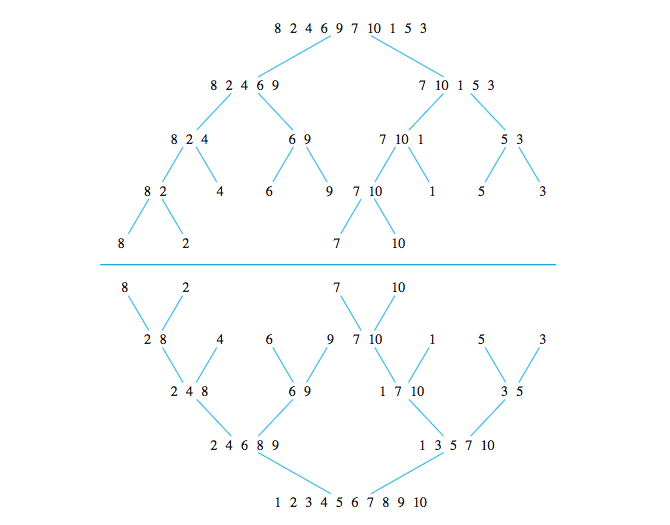
\includegraphics[scale = 0.45]{mergesort}$$ \end{example} 

In general, a merge sort proceeds by iteratively splitting lists into two sublists of equal length (or where one sublist has one more element than the other) until each sublist contains one element. This succession of sublists can be represented by a balanced binary tree. The procedure continues by successively merging pairs of lists, where both lists are in increasing order, into a larger list with elements in increasing order, until the original list is put into increasing order. The succession of merged lists can be represented by a balanced binary tree. 
\begin{alg} Recursive Merge Sort \\ 
procedure \textit{mergesort}($L = a_1, \dots, a_n$) \\ 
if $n > 1$ then \\ 
\indent $m := \lfloor n/2 \rfloor $ \\
\indent $L_1 := a_1, a_2, \dots, a_m$ \\ 
\indent $L_2 := a_{m + 1}, a_{m + 2}, \dots, a_n$ \\ 
\indent $L := merge(mergesort(L_1), mergesort(L_2))$ \\ 
\{$L$ is now sorted into elements in nondecreasing order.\} \end{alg} 

\begin{example} Merge the two lists 2, 3, 5, 6 and 1, 4. \\ 
First, compare the smallest elements in the two lists, 2 and 1, respectively. Because 1 is the smaller, put it at the beginning of the merged list and remove it from the second list. At this stage, the first list is 2, 3, 5, 6, the second list is 4, and the combined list is 1. \\ Next, compare 2 and 4, the smallest elements of the two lists. Because 2 is the smaller, add it to the combined list and remove it from the first list. At this stage, the first list is 3, 5, 6, the second is 4 and the combined list is 1, 2. \\ Continue by comparing 3 and 4, the smallest elements of their respective lists. Because 3 is the smaller of these two elements, add it to the combined list and remove it from the first list. At the stage, the first list is 5, 6, and the second list is 4. The combined list is 1, 2, 3. \\ Then compare 5 and 4, the smallest elements in the two lists. Because 4 is the smaller of these two elements, add it to the combined list and remove it from the second list. At this stage, the first list is 5, 6, the second list is empty and the combined list is 1, 2, 3, 4. \\ Finally, because the second list is empty, all elements of the first list can be appended to the end of the combined list in the order they appear in the first. This produces the ordered list 1, 2, 3, 4, 5, 6. 
$$\begin{tabular}{|c|c|c|c|} \hline First list & Second List & Merged List & Comparison \\ \hline 2 3 5 6 & 1 4 & & 1 $<$ 2 \\ \hline 2 3 5 6 & 4 & 1 & 2 $<$ 4 \\ \hline 3 5 6 & 4 & 1 2 & 3 $<$ 4 \\ \hline 5 6 & 4 & 1 2 3 & 4 $<$ 5 \\ \hline 5 6 & & 1 2 3 4 & \\ \hline & & 1 2 3 4 5 6 & \\ \hline \end{tabular} $$ \end{example} 
Each time a comparison of an element from $L_1$ and an element from $L_2$ is made, an additional element is added to the merged list $L$. However, when either $L_1$ or $L_2$ is empty, no more comparisons are needed. Hence, merging two lists is least efficient when $m + n - 2$ comparisons are carried out, where $m$ and $n$ are the number of elements in $L_1$ and $L_2$ respectively, leaving one element in each of $L_1$ and $L_2$. The next comparison will be the last one needed, because it will make one of these lists empty. Therefore, merging two lists uses no more than $m + n - 1$ comparisons. 
\begin{alg} Merging Two Lists \\ 
procedure \textit{merge}($L_1, L_2$: sorted lists) \\ 
$L$: = empty list \\ 
while $L_1$ and $L_2$ are both nonempty \\ 
\indent remove smaller of first elements of $L_1$ and $L_2$ from its list; put it at the first end of $L$ \\
\indent if this remove makes one list empty, then remove all elements from the other list and append them to $L$ \\ 
return $L$\{$L$ is the merged list with elements in increasing order\} \end{alg} 
\begin{theorem} Two sorted lists with $m$ elements and $n$ elements can be merged into a sorted list using no more than $m + n - 1$ comparisons. \end{theorem} 
Analyze the complexity of the merge sort. Assume that $n$, the number of elements in the list, is a power of 2, say $2^m$. At the first stage of the splitting procedure, the list is split into two sublists, of $2^{m - 1}$ elements each, at level 1 of the tree generated by the splitting. This procedure continues, splitting the two sublists with $2^{m - 1}$ elements into four sublists of $2^{m - 2}$ elements, each at level 2, and so on. In general, there are $2^{k - 1}$ lists at level $k - 1$, each with $2^{m - k + 1}$ elements. These lists at level $k - 1$ are split into $2^k$ lists at level $k$, each with $2^{m - k}$ elements. At the end of this process, there are $2^m$ lists each with one elements at level $m$. Start merging by combining pairs of the $2^m$ lists of one element into $2^{m - 1}$ lists, at level $m - 1$, each with two elements .To do this, $2^{m - 1}$ pairs of lists with one element are merged. The merger of each pair requires exactly one comparison. The procedure continues, so that at level $k$ ($k = m, m - 1, m - 2, \dots, 3, 2, 1$), $2^k$ lists each with $2^{m - k}$ elements are merged into $2^{k - 1}$ lists, each with $2^{m - k + 1}$ elements, at level $k - 1$. To do this a total of $2^{k - 1}$ mergers of two lists, each with $2^{m - k}$ elements, are needed. But each of these mergers can be carried out using at most $2^{m - k} + 2^{m - k} - 1 = 2^{m - k + 1} - 1$ comparisons. Hence, going from level $k$ to $k - 1$ can be accomplished using at most $2^{k - 1}(2^{m - k + 1} - 1)$ comparisons. Summing all these estimates shows that the number of comparisons required for the merge sort is at most $$\sum_{k = 1}^m 2^{k - 1}(2^{m - k + 1} - 1) = \sum_{k = 1}^m 2^m - \sum_{k = 1}^m 2^{k - 1} = m2^m - (2^m - 1) = n\log n - n + 1$$ because $m = \log n$ and $n = 2^m$. 
\begin{theorem} The number of comparisons needed to merge sort a list with $n$ elements is $O(n\log n)$. \end{theorem} 

\section{Advanced Counting Techniques}
\subsection{Applications of Recurrence Relations} 
\begin{definition} Recurrence Relation: an equation that expresses $a_n$ in terms of one or more of the previous terms of the sequence, namely, $a_0, a_1, \dots, a_{n - 1}$, for all integers $n$ with $n \geq n_0$, where $n_0$ is a nonnegative integer \end{definition} 
\begin{example} A young pair of rabbits (one of each sex) is placed on an island. A pair of rabbits does not breed until they are 2 months old. After they are 2 months old, each pair of rabbits produces another pair each month. Find a recurrence relation for the number of pairs of rabbits on the island after $n$ months, assuming that no rabbits ever die. $$\begin{tabular}{|c|c|c|c|c|c|} \hline Reproducing Pairs & Young Pairs & & Reproducing & Young & Total \\ (at least 2 months old) & (less than two months old) & Month & pairs & pairs & pairs \\ \hline 0 & 2 & 1 & 0 & 1 & 1 \\ \hline 0 & 2 & 2 & 0 & 1 & 1 \\ \hline 2 & 2 & 3 & 1 & 1 & 2 \\ \hline 2 & 4 & 4 & 1 & 2 & 3 \\ \hline 4 & 6 & 5 & 2 & 3 & 5 \\ \hline 6 & 10 & 6 & 3 & 2 & 8 \\ \hline \end{tabular} $$ 
Denote by $f_n$ the number of pairs of rabbits after $n$ months. The rabbit population can be modeled using a recurrence relation. At the end of the first month, the number of pairs of rabbits on the island is $f_1 = 1$. Because this pair does not breed during the second month, $f_2 = 1$ also. To find the number of pairs after $n$ months, add the number on the island the previous month, $f_{n - 1}$, and the number of newborn pairs, which equals $f_{n - 2}$, because each newborn pair comes from a pair at least 2 months old. Consequently, the sequence $\{f_n\}$ satisfies the recurrence relation $$f_n = f_{n - 1} + f_{n - 2}$$ for $n \geq 3$ together with the initial conditions $f_1 = 1$ and $f_2 = 1$. Because this recurrence relation and the initial condition uniquely determine this sequence, the number of pairs of rabbits on the island after $n$ months is given by the $n$th Fibonacci number. \end{example} 

\begin{example} A popular puzzle of the late nineteenth century, called the Tower of Hanoi, consists of three pegs mounted on a board together with disk of different sizes. Initially these disks are placed on the first peg in order of size, with the largest on the bottom. The rules of the puzzle allow disks to be moved one at a time from one peg to another as long as a disk is never placed on top of a smaller disk. The goal of the puzzle is to have all the disks on the second peg in order of size, with the largest on the bottom. Let $H_n$ denote the number of moves needed to solve the Tower of Hanoi problem with $n$ disks. Set up a recurrence relation for the sequence $\{H_n\}$. \\~\\ 
Begin with $n$ disks on peg 1.Transfer the top $n - 1$ disks, following the rules of the puzzle, to peg 3 using $H_{n - 1}$ moves. Keep the largest disk fixed during these moves. Then, use one move to transfer the largest disk to the second peg. Transfer the $n - 1$ disks on peg 3 to peg 2 using $H_{n - 1}$ additional moves, placing them on top of the largest disk, which always stays fixed on the bottom of peg 2. It is easy to see that the puzzle cannot be solved using fewer steps. This shows that $$H_n = 2H_{n - 1} + 1$$ 
The initial condition is $H_1 = 1$, because one disk can be transferred from peg 1 to peg 2, according to the rules of the puzzle, in one move. To solve the recurrence relation, use an iterative approach. Note that $$\begin{aligned} H_n &= 2H_{n - 1} + 1 \\ &= 2(2H_{n - 2} + 1) + 1 = 2^2 H_{n - 2} + 2 + 1 \\ &= 2^2(2H_{n - 2} + 1) + 2 + 1 = 2^3H_{n - 3} + 2^2 + 2 + 1 \\ &\vdots \\ &= 2^{n - 1}H_1 + 2^{n - 2} + 2^{n - 3} + \dots + 2 + 1 \\ &= 2^{n - 1} + 2^{n - 2} + \dots + 2 + 1 \\ &= 2^n - 1 \end{aligned} $$ 
Here the recurrence relation was used repeatedly to express $H_n$ in terms of previous terms of the sequence. In the next to last equality, the initial condition $H_1 = 1$ has been used. The last equality is based on the formula for the sum of the terms of a geometric series. $$ \sum_{j = 0}^n ar^j = \begin{cases} \frac{ar^{n + 1} - a}{r - 1} &\text{ if } r \neq 1 \\ (n + 1)a &\text{ if } r = 1 \end{cases} $$ The iterative approach has produced the solution to the recurrence relation $H_n = 2H_{n - 1} + 1$ with the initial condition $H_1 = 1$. \\~\\ A myth created to accompany the puzzle tells of a tower in Hanoi where monks are transferring 64 gold disks from one peg to another, according to the rules of the puzzle. The myth says that the world will end when they finish the puzzle. How long after the monks started will the world end if the monks take one second to move a disk? \\ From the explicit formula, the monks require $$ 2^{64} - 1 = 18,446,744,073,709,551,615 $$ moves to transfer the disks. Making one move per second, it would take them more than 500 billion years to complete the transfer, so the world should survive a while longer than it already has. \end{example} 

\begin{example} Find a recurrence relation and give initial conditions for the number of bit strings of length $n$ that do not have two consecutive 0s. How many such bit strings are there of length 5? \\~\\ 
Let $a_n$ denote the number of bit strings of length $n$ that do not have two consecutive 0s. To obtain a recurrence relation for $\{a_n\}$, note that by the sum rule, the number of bit strings of length $n$ that do not have two consecutive 0s equals the numbers of such bit strings ending with a 0 plus the number of such bit strings ending with a 1. Assume that $n \geq 3$, so that the bit string has at least 3 bits. \\
The bit strings of length $n$ ending with 1 that do not have two consecutive 0s are precisely the bit strings of length $n - 1$ with no two consecutive 0s with a 1 added in the end. Consequently, there are $a_{n - 1}$ such bit strings. \\~\\ Bit strings of length $n$ ending a 0 that do not have two consecutive 0s must have 1 as their $(n - 1)$st bit; otherwise they would end with a pair of 0s. It follows that the bit strings of length $n$ ending a 0 that have no two consecutive 0s are precisely the bit strings of length $n - 2$ with no two consecutive 0s with 10 added at the end. Consequently, there are $a_{n - 2}$ such bit strings. Conclude that $$a_n = a_{n - 1} + a_{n - 2} $$ for $n \geq 3$. The initial conditions are $a_1 = 2$, because both bit strings of length one, 0 and 1 do not have consecutive 0s, and $a_2 = 3$, because the valid bit strings of length two are 01, 10, and 11. To obtain $a_5$, use the recurrence relation to find that $$\begin{aligned} a_3 &= a_ 2 + a_1 = 3 + 2 = 5 \\ a_4 &= a_3 + a_2 = 5 + 3 = 8 \\ a_5 &= a_4 + a_3 = 8 + 5 = 13 \end{aligned} $$ Note that $\{a_n\}$ satisfies the same recurrence relation as the Fibonacci sequence. Because $a_1 = f_3$ and $a_2 = f_4$, it follows that $a_n = f_{n + 2}$. \end{example} 

\begin{example}
Find a recurrence relation for the number of strictly increasing sequence of positive integers that have 1 as their first term and $n$ as their last term, where $n$ is a positive integer. That is, sequences $a_1, a_2, \dots, a_k$, where $a_1 = 1$, $a_k = n$ and $a_j < a_{j + 1}$ for $j = 1, 2, \dots, k - 1$. 
$$ \begin{aligned} a_1 &= \{1\} \\ a_2 &= \{1, 2\} \\ a_3 &= \{1, 3\}, \{1, 2, 3\} \\ a_4 &= \{1, 4\}, \{1, 2, 4\}, \{1, 3, 4\}, \{1, 2, 3, 4\}  \\ a_5 &= \{1, 5\}. \{1, 2, 5\}, \{1, 3, 5\}, \{1, 4, 5\}, \{1, 2, 3, 5\}, \{1, 2, 4, 5\}, \{1, 3, 4, 5\}, \{1, 2, 3, 4, 5\} \end{aligned} $$ 
$$ \begin{tabular}{|c|c|} \hline \\ $n$ & Number of Sequences \\ \hline 
2 & 1 \\ \hline 3 & 2 \\ \hline 4 & 4 \\ \hline 5 & 8 \\ \hline 6 & 16 \\ \hline \end{tabular} $$  
$$a_n = 2^{n - 2} $$\end{example} 

\begin{example} Example 10. Find the recurrence relation for the number of strings of length $n$ that contain the string 01. What are the initial conditions? How many bit strings of length seven contain 01? \\ 
Let $a_n$ be the number of bit strings of length $n$ that contain the string 01. To construct such a string, start with a 1 and follow it with a bit string of length $n - 1$ that contains 01, and there are $a_{n - 1}$ of these. Alternatively, for any $k$ from 1 to $n - 1$, start with $k$ 0s, follow this by a 1, and then follow this by any $n - k - 1$ bits. For each such $k$, there are $2^{n - k - 1}$ such strings, since the final bits are free. Therefore the number of such strings is $2^0 + 2^1 + 2^2 + \dots + 2^{n - 2}$, which equals $2^{n - 1} - 1$. Thus $$a_n = a_{n - 1} + 2^{n - 1} - 1 $$ 
The initial conditions are $a_0 = a_1 = 0$, since no string of length less than 2 can have 01 in it. 
$$\begin{aligned}
 a_0 &= 0 \\ a_1 &= 0 \\ a_2 &= a_1 + 2^1 - 1 = 0 + 2 - 1 = 1 \\ a_3 &= a_2 + 2^2 - 1 = 1 + 4 - 1 = 4 \\ a_4 &= a_3 + 2^3 - 1 = 4 + 8 - 1 = 11 \\ a_5 &= a_4 + 2^4 - 1 = 11 + 16 - 1 = 26 \\ a_6 &= a_5 + 2^5 - 1 = 26 + 32 - 1 = 57 \\ a_7 &= a_6 + 2^6 - 1 = 57 + 64 - 1 = 120 \end{aligned} $$ \end{example} 

\begin{example} A computer system considers a string of decimal digits a valid codeword if it contains an even number of 0 digits. For example, 1230407869 is valid, whereas 120987045608 is not valid. Let $a_n$ be the number of valid $n$-digit codewords. Find a recurrence relation for $a_n$. \\ Note that $a_1 = 9$ because there are 10 one-digit strings, and only one, namely, the string 0, is not valid. A recurrence relation can be derived for this sequence by considering how a valid $n$-digit string can be obtained from strings of $n - 1$ digits. There are two ways to form a valid string with $n$ digits from a string with one fewer digits. \\ First, a valid string of $n$ digits can be obtained by appending a valid string of $n - 1$ digits with a digit other than 0. This appending can be done in nine ways. Hence, a valid string with $n$ digits can be formed in this manner in $9a_{n - 1}$ ways. \\ Second, a valid string of $n$ digits can be obtained by appending a 0 to a string of length $n - 1$ that is not valid. This produces a string with an even number of 0 digits because the invalid string of length $n - 1$ has an odd number of 0 digits. The number of ways that this can be done equals the number of invalid $(n - 1)$-digit strings. Because there are $10^{n - 1}$ strings of length $n - 1$, and $a_{n - 1}$ are valid, there are $10^{n - 1} - a_{n - 1}$ valid $n$- digit strings obtained by appending an invalid string of length $n - 14$ with a 0. \\ 
Thus $$\begin{aligned} a_n &= 9a_{n - 1} + (10^{n - 1} - a_{n - 1}) \\ &= 8a_{n - 1} + 10^{n - 1} \end{aligned} $$ \end{example} 

\subsection{Solving Linear Recurrence Relations}

\begin{definition} A linear homogeneous recurrence relation of degree $k$ with constant coefficients is a recurrence relation of the form $$a_n = c_1a_{n - 1} + c_2a_{n - 2} + \dots + c_ka_{n - k} $$ where $c_1, c_2, \dots, c_k$ are real numbers and $c_k \neq 0$. \end{definition} 

The recurrence relation in the definition above is linear because the RHS is a sum of previous terms of the sequence each multiplied by a function of $n$> The recurrence relation is homogeneous because no terms occur that are not multiples of the $a_j$s. The coefficients of the terms of the sequence are all constants, rather than functions that depend on $n$. The degree is $k$ because $a_n$ is expressed in terms of the previous $k$ terms of the sequence. \\~\\ 
The basic approach for solving linear homogeneous recurrence relations is to look for solutions of the form $a_n = r^n$ where $r$ is a constant. Note that $a_n = r^n$ is a solution of the recurrence relation $a_n = c_1a_{n - 1} + c_2a_{n - 2} + \dots + c_ka_{n - k} $ if and only if $$r^n = c_1r^{n - 1} + c_2r^{n - 2} + \dots + c_kr^{n - k} $$ When both sides of the equation are divided by $r^{n - k}$ and the RHS is subtracted from the left, the following equation is obtained $$r^k - c_1r^{k - 1} - c_2r^{k - 2} - \dots - c_{k - 1}r - c_k = 0 $$ 
\begin{theorem} Let $c_1$ and $c_2$ be real numbers. Suppose that $r^2 - c_1r - c_2 = 0$ has two distinct roots $r_1$ and $r_2$>  Then the sequence $\{a_n\}$ is a solution of the recurrence relation $a_n = c_1a_{n - 1} + c_2a_{n - 2}$ if and only if $$a_n = \alpha_1r_1^n + \alpha_2r_2^n$$ for $n = 0, 1, 2, \dots$ where $\alpha_1$ and $\alpha_2$ are constants. \end{theorem}

\begin{example} What is the solution of the recurrence relation $$a_n = a_{n - 1} + 2a_{n - 2} $$ with $a_0 = 2$ and $a_1 = 7$? \\ The characteristic equation of the recurrence relation is $r^2 - r - 2 = 0$. Its roots are $r = 2$ and $r = -1$. Hence, the sequence $\{a_n\}$ is a solution to the recurrence relation if and only if $$a_n = \alpha_12^n + \alpha_2(-1)^n $$ for some constants $\alpha_1$ and $\alpha_2$. From the initial conditions, it follows that $$\begin{aligned} a_0 &= 2 = \alpha_1 + \alpha_2 \\ a_1 &= 7 = 2\alpha_1 + (-1)\alpha_2 \end{aligned} $$ Solving these two equations show that $\alpha_1 = 3$ and $\alpha_2 = -1$. Hence the solution to the recurrence relation and initial conditions is the sequence $\{a_n\}$ with $$a_n = 3\cdot 2^n - (-1)^n $$ \end{example} 

\begin{example} Find an explicit formula for the Fibonacci numbers. \\ Recall that the sequence of Fibonacci numbers satisfies the recurrence relation $f_n = f_{n - 1} + f_{n - 2}$ and also satisfies the initial conditions $f_0 = 0$ and $f_1 = 1$> The roots of the characteristic equation $r^2 - r - 1 = 0$ are $r_1 = \frac{1 + \sqrt{5}}{2}$ and $r_2 = \frac{1 - \sqrt{5}}{2} $, Therefore, it follows that the Fibonacci numbers are given by $$f_n = \alpha_1\Big(\frac{1 + \sqrt{5}}{2}\Big)^n + \alpha_2\Big(\frac{1 - \sqrt{5}}{2}\Big)^n $$ for some constants $\alpha_1$ and $\alpha_2$. The initial conditions $f_0 = 0$ and $f_1 = 1$ can be used to find these constants. $$\begin{aligned} f_0 &= \alpha_ 1 + \alpha_2 = 0 \\ f_1 &= \alpha_1\Big(\frac{1 + \sqrt{5}}{2}\Big) + \alpha_2\Big(\frac{1 - \sqrt{5}}{2}\Big) = 1 \end{aligned} $$ The solutions to these simultaneous equations for $\alpha_1$ and $\alpha_2$ is $$\begin{aligned} \alpha_1 &= \frac{1}{\sqrt{5}} \\ \alpha_2 &= -\frac{1}{\sqrt{5}} \end{aligned} $$ Thus the Fibonacci numbers are given by $$f_n = \frac{1}{\sqrt{5}}\Big( \frac{1 + \sqrt{5}}{2}\Big)^n - \frac{1}{\sqrt{5}}\Big(\frac{ 1 - \sqrt{5}}{2}\Big)^n $$ \end{example}
Note: The above theorem does not apply then there is one characteristic root of multiplicity two. 
\begin{theorem} Let $c_1$ and $c_2$ be real numbers with $c_2 \neq 0$. Suppose that $r^2 - c_1r - c_2 = 0$ has only one root $r_0$. A sequence $\{a_n\}$ is a solution of the recurrence relation $a_n = c_1a_{n - 1} + c_2a_{n - 2}$ if and only if $$ a_n = \alpha_1r_0^n + \alpha_2nr_0^n $$ for $n = 0, 1, 2, \dots$, where $\alpha_1$ and $\alpha_2$ are constants. \end{theorem} 

\begin{example} What is the solution of the recurrence relation $$a_n = 6a_{n - 1} - 9a_{n - 2} $$ with initial conditions $a_0 = 1$ and $a_1 = 6$? \\ The only root of $r^2 - 6r + 9 = 0$ is $r = 3$. Hence, the solution to this recurrence relation is $$a_n = \alpha_13^n + \alpha_2n3^n $$ for some constants $\alpha_1$ and $\alpha_2$. Using the initial conditions, it follows that 
$$\begin{aligned} a_0 &= 1 = \alpha_1 \\ a_1 &= 6 = 3\alpha_1 + 3\alpha_2 \end{aligned} $$ Solving these two equations shows that $\alpha_ 1 = 1$ and $\alpha_2 = 1$. Consequently, the solution to this recurrence relation and the initial conditions is $$a_n = 3^n + n3^n $$ \end{example} 

\begin{theorem} Let $c_1, c_2, \dots, c_k$ be real numbers. Suppose that the characteristic equation $$r^k - c_1r^{k - 1} - \dots - c_k = 0$$ has $k$ distinct roots $r_1, r_2, \dots, r_k$. Then a sequence $\{a_n\}$ is a solution of the recurrence relation $$a_n = c_1a_{n - 1} + c_2a_{n - 2} + \dots + c_ka_{n - k} $$ if and only if $$a_n = \alpha_1r_1^n + \alpha_2r_2^n + \dots + \alpha_kr_k^n $$ for $n = 0, 1, 2, \dots,$ where $\alpha_1, \alpha_2, \dots, \alpha_k$ are constants. \end{theorem} 

\begin{example} Find the solution to the recurrence relation $$a_n = 6a_{n - 1} - 11a_{n - 2} + 6a_{n - 3} $$ with the initial conditions $a_0 = 2$, $a_1 = 5$ and $a_2 = 15$. \\ 
The characteristic polynomial of this recurrence relation is $$r^3 - 6r^2 + 11r - 6 = 0 $$ The characteristics roots are $r = 1$, $r = 2$ and $r = 3$, because $r^3 - 6r^2 + 11r - 6 = (r - 1)(r - 2)(r - 3)$. Hence the solutions to this recurrence relation are of the form $$a_n = \alpha_1\cdot 1^n + \alpha_2 \cdot 2^n + \alpha_3 \cdot 3^n $$ To find the constants, use the initial conditions. 
$$\begin{aligned} a_0 &= 2 = \alpha_1 + \alpha_2 + \alpha_3 \\ a_1 &= 5 = \alpha_1 + 2\alpha_2 + 3\alpha_3 \\ a_2 &= 15 = \alpha_1 + 4\alpha_2 + 9\alpha_3 \end{aligned} $$ Therefore $\alpha_1 = 1$, $\alpha_2 = -1$ and $\alpha_3 = 2$. Thus, the unique solution to this recurrence relation and the given initial conditions is the sequence $\{a_n\}$ with $$a_n = 1 - 2^n + 2\cdot 3^n $$ \end{example} 

\begin{theorem} Let $c_1, c_2, \dots, c_k$ be real numbers. Suppose that the characteristic equation $$r^k - c_1r^{k - 1} - \dots - c_k = 0$$ has $t$ distinct roots $r_1, r_2, \dots, r_t$ with multiplicities $m_1, m_2, \dots, m_t$, respectively, so that $m_i \geq 1$ for $i = 1, 2, \dots, t$and $m_1 + m_2 + \dots + m_t = k$. Then a sequence $\{a_n\}$ is a solution of the recurrence relation $$a_n = c_1a_{n - 1} + c_2a_{n - 2} + \dots + c_ka_{n - k} $$ if and only if $$ \begin{aligned} 
a_n &= (\alpha_{1, 0} + \alpha_{1, 1}n + \dots + \alpha_{1, m_1 - 1}n^{m_1 - 1})r_1^n \\ &+ (\alpha_{2, 0} + \alpha_{2, 1}n + \dots + \alpha_{2, m_2 - 1}n^{m_2 - 1})r_2^n \\ &+ \dots + (\alpha_{t, 0} + \alpha_{t, 1}n + \dots + \alpha_{t, m_t - 1}n^{m_t - 1})r_t^n \end{aligned} $$ for $n = 0, 1, 2, \dots,$ where $\alpha_{i, j}$ are constants for $1 \leq i \leq t$ and $0 \leq j \leq m_i - 1$. \end{theorem} 

\begin{example} Suppose that the roots of the characteristic equation of a linear homogeneous recurrence relation are 2, 2, 2, 5, 5, and 9 (that is, there are three roots, the root 2 with multiplicity three, the root 5 with multiplicity two, and the root 9 with multiplicity one). What is the form of the general solution? 
$$(\alpha_{1, 0} + \alpha_{1, 1}n + \alpha_{1, 2}n^2)2^n + (\alpha_{2, 0} + \alpha_{2, 1}n)5^n + \alpha_{3, 0}9^n $$ \end{example} 

\begin{example} Find the solution to the recurrence relation $$a_n = -3a_{n - 1} - 3a_{n - 2} - a_{n - 3} $$ with initial conditions $a_0 = 1$, $a_1 = -2$ and $a_2 = -1$. \\ The characteristic equation of this recurrence relation is $$r^3 + 3r^2 + 3r + 1 = 0 $$ Because $r^3 + 3r^2 + 3r  + 1 = (r + 1)^3$, there is a single root $r = -1$ of multiplicity three of the characteristic equation. Thus the solutions of this recurrence relation are of the form $$a_n = \alpha_{1, 0}(-1)^n + \alpha_{1, 1}n(-1)^n + \alpha_{1, 2}n^2(-1)^n $$ To find the constants, use the initial conditions, $$\begin{aligned} a_0 &= 1 = \alpha_{1, 0} \\ a_1 &= -2 = -\alpha_{1, 0} - \alpha_{1, 1} - \alpha_{1, 2} \\ a_2 &= -1 = \alpha_{1, 0} + 2\alpha_{1, 1} + 4\alpha_{1, 2} \end{aligned} $$ 
The simultaneous solution of these three equations is $\alpha_{1, 0} = 1$, $\alpha_{1, 1} = 3$ and $\alpha_{1, 2} = -2$. Hence the unique solution to this recurrence relation and the given initial conditions is the sequence $\{a_n\}$ with $$a_n = (1 + 3n - 2n^2)(-1)^n $$ \end{example}

\begin{definition} Linear Nonhomogenous Recurrence Relation with Constant Coefficients: a recurrence relation of the form $$a_n = c_1a_{n - 1} + c_2a_{n - 2} + \dots + c_ka_{n - k} + F(n)$$ where $c_1, c_2, \dots, c_k$ are real numbers and $F(n)$ is a function not identically zero depending on $n$. \end{definition} 
\begin{definition} Associated Homogeneous Recurrence Relation: $$ a_n = c_1a_{n - 1} + c_2a_{n - 2} + \dots + c_ka_{n - k} $$ \end{definition}

\begin{example} Each of the recurrence relations $a_n = a_{n - 1} + 2^n$, $a_n = a_{n - 1} + a_{n - 2} + n^2 + n - 1$, $a_n = 3a_{n -1} + n3^n$ and $a_n = a_{n - 1} + a_{n - 2} + a_{n - 3} + n!$ is a linear nonhomogeneous recurrence relation with constant coefficients. The associated linear homogeneous recurrence relations are $a_n = a_{n - 1}$, $a_n = a_{n - 1} + a_{n - 2}$, $a_n = 3a_{n - 1}$ and $a_n = a_{n - 1} + a_{n - 2} + a_{n - 3}$, respectively. \end{example} 

\begin{theorem} If $\{a_n^{(p)}\}$ is a particular solution of the nonhomogeneous linear recurrence relation with constant coefficients $$a_n = c_1a_{n - 1} + c_2a_{n - 2} + \dots + c_ka_{n - k} + F(n)$$ then every solution is of the form $$\{a_n^{(p)} + a_n^{(h)}\} $$ where $\{a_n^{(h)}\}$ is a solution of the associated homogeneous recurrence relation $$a_n = c_1a_{n -1} + c_2a_{n - 2} + \dots + c_ka_{n - k} $$ \end{theorem} 

\begin{example} Find all solutions of the recurrence relation $$a_n = 3a_{n - 1} + 2n$$ What is the solution with $a_1 = 3$? \\ 
To solve this linear nonhomogeneous recurrence relation with constant coefficients, solve its associated linear homogeneous equation. The associated linear homogeneous equation is $$a_n = 3a_{n - 1}$$ Its solutions are $a_n^{(h)} = \alpha3^n $ where $\alpha$ is a constant. \\~\\
Now find a particular solution. Because $F(n) = 2n$ is a polynomial in $n$ of degree one, a reasonable trial solution is a linear function in $n$, say, $p_n = cn + d$, where $c$ and $d$ are constants, to determine whether there are any solutions of this form, suppose that $p_n = cn + d$ is such a solution. Then $$a_n = 3a_{n - 1} + 2n = 3(c(n - 1) + d) + 2n $$ Simplifying and combining like terms gives $$(2 + 2c)n + (2d - 3c) = 0$$ It follows that $cn + d$ is a solution if and only if $2 + 2c = 0$ and $2d - 3c = 0$. This shows that $cn + d$ is a solution if and only if $c = -1$ and $d = -\frac{3}{2}$. Consequently, $a_n^{(p)} = -n - \frac{3}{2} $ is a particular solution. Therefore, all solutions are of the form $$a_n = a_n^{(p)} + a_n^{(h)} = -n - \frac{3}{2} + \alpha \cdot 3^n $$ where $\alpha$ is a constant. \\~\\ To find the solution with $a_1 = 3$, let $n = 1$ in the formula above. Then $$ 3 = -1 - \frac{3}{2} + 3\alpha$$ which implies that $\alpha = \frac{11}{6}$. Therefore the solution is $$a_n = -n - \frac{3}{2} + \Big(\frac{11}{6}\Big)3^n $$ \end{example} 

\begin{example} Find all solutions of the recurrence relation $$a_n = 5a_{n - 1} - 6a_{n - 2} + 7^n$$ 
This is a linear nonhomogeneous recurrence relation. The solution of its associated homogeneous recurrence relation $$a_n = 5a_{n - 1} - 6a_{n - 2} $$ are $a_n^{(h)} = \alpha_1 \cdot 3^n + \alpha_2 \cdot 2^n$ where $\alpha_1$ and $\alpha_2$ are constants. Because $F(n) = 7^n$, a reasonable trial solution is $a_n^{(p)} = C \cdot 7^n$ where $C$ is a constant. Substituting the terms of this sequence into the recurrence relation implies that $$C \cdot 7^n = 5C \cdot 7^{n - 1} - 6C \cdot 7^{n - 2} + 7^n $$ Factoring out $7^{n - 2}$, this equation becomes $49C = 35C - 6C + 49$, which implies that $20C = 49$, or that $C = \frac{49}{20}$. Hence $a_n^{(p)} = \Big(\frac{49}{20}\Big)7^n$ is a particular solution. Thus all solutions are of the form $$a_n = \alpha_1 \cdot 3^n + \alpha_2 \cdot 2^n + \Big( \frac{49}{20}\Big)7^n $$ \end{example} 

\begin{theorem} Suppose that $\{a_n\}$ satisfies the linaer nonhomogeneous recurrence relation $$a_n = c_1a_{n - 1} + c_2a_{n - 2} + \dots+ c_ka_{n - k} + F(n)$$ where $c_1, c_2, \dots, c_k$ are real numbers, and $$F(n) = (b_tn^t + b_{t - 1}n^{t - 1} + \dots + b_1n + b_0)s^n $$ where $b_0, b_1, \dots, b_t$ and $s$ are real numbers. When $s$ is not a root of the characteristic equation of the associated linear homogeneous recurrence relation, there is a particular solution of the form $$(p_tn^t + p_{t - 1}n^{t - 1} + \dots + p_1n + p_0)s^n$$ When $s$ is a root of this characteristic equation and its multiplicity is $m$, there is a particular solution of the form $$n^m(p_tn^t + p_{t - 1}n^{t - 1} + \dots + p_1n + p_0)s^n $$ \end{theorem} 

\begin{example} What form does a particular solution of the linear nonhomogeneous recurrence relation $$a_n = 6a_{n - 1} - 9a_{n - 2} + F(n)$$ have when $F(n) = 3^n$, $F(n) = n3^n$, $F(n) = n^22^n$, and $F(n) = (n^2 + 1)3^n$? \\ 
The associated linear homogeneous recurrence relation is $$a_n = 6a_{n - 1} - 9a_{n - 2} $$ Its characteristic equation $r^2 - 6r + 9 = (r - 3)^2 = 0$, has a single root, 3, of multiplicity two. To apply the above theorem, with $F(n)$ of the form $P(n)s^n$, where $P(n)$ is a polynomial and $s$ is a constant, ask whether $s$ is a root of this characteristic equation. \\~\\ 
Because $s = 3$ is a root with multiplicity $m = 2$ but $s = 2$ is not a root, the above theorem tells us that a particular solution has the form $p_0n^23^n$ if $F(n) = 3^n$, the form $n^2(p_1n + p_0)3^n$ if $F(n) = n3^n$, the form $(p_2n^2 + p_1n + p_0)2^n$ if $F(n) = n^22^n$, and the form $n^2(p_2n^2 + p_1n + p_0)3^n$ if $F(n) = (n^2 + 1)3^n$. \end{example} 

When $s = 1$, with $F(n) = b_tn_t + b_{t - 1}n_{t  - 1} + \dots + b_1n + b_0$, the parameter $s$ takes the value $s = 1$. By the theorem, the form of the solution then depends on whether 1 is a root of the characteristic equation of the associated linear homogeneous recurrence relation. 

\begin{example} Let $a_n$ be the sum of the first $n$ positive integers, so that $$a_n = \sum_{k = 1}^n k $$ Note that $a_n$ satisfies the linear nonhomgeneous recurrence relation $$a_n = a_{n - 1} + n $$ Note that the initial condition is $a_1 = 1$. The associated linear homogeneous recurrence relation for $a_n$ is $$ a_n = a_{n - 1} $$ The solutions of this homogeneous recurrence relation are given by $a_n^{(h)} = c(1)^n = c$, where $c$ is a constant. To find all solutions of $a_n = a_{n - 1} + n$, find only a single particular solution. Because $F(n) = n = n \cdot (1)^n$ and $s = 1$ is a root of degree one of the characteristic equation of the associated linear homogeneous recurrence relation, there is a particular solution of the form $n(p_1n + p_0) = p_1n^2 + p_0n $. Inserting this into the recurrence relation gives $$p_1n^2 + p_0n = p_1(n - 1)^2 + p_0(n - 1) + n $$ Simplifying, $$n(2p_1 - 1) + (p_0 - p_1) = 0$$ which means that $2p_1 - 1 = 0$ and $p_0 - p_1 = 0$, so $p_0 = p_1 = \frac{1}{2}$. Therefore $$a_n^{(p)} = \frac{n^2}{2} + \frac{n}{2} = \frac{n(n + 1)}{2} $$ is a particular solution. Hence, all solutions of the original recurrence relation $a_n = a_{n - 1} + n$ are given by $a_n = a_n^{(h)} + a_n^{(p)} = c + \frac{n(n + 1)}{2} $. Because $a_1 = 1$, $1 = a_1 = c + 1 \cdot \frac{2}{2} = c + 1$, so $c = 0$. It follows that $$ a_n = \frac{n(n + 1)}{2} $$ \end{example} 

\begin{example} A vending machine dispensing books of stamps accepts only one-dollar coins, \$1 bills, and \$5 bills. Find a recurrence relation for the number of ways to deposit $n$ dollars in the vending machine, where the order in which the coins and bills are deposited matters. What are the initial conditions? How many ways are there to deposit \$10 for a book of stamps?
$$ a_n = 2a_{n - 1} + a_{n - 5} $$
Initial Condition: $a_0 = 1$, $a_{-1} = a_{-2} = a_{-3} = a_{-4} = a_{-5} = 0 $ $$\begin{aligned}
a_1 &= 2a_0 + a_{-5} = 2 \\
a_2 &= 2a_1 + a_{-4}  = 4 \\
a_3 & = 2a_2  + a_{-3} = 8 \\
a_4 & = 2a_3 + a_{-2} = 16 \\
a_5 & = 2a_4 + a_{-1} = 32 \\
a_6 & = 2a_5 + a_0 = 2 \cdot 32 + 1 = 65 \\
a_7 & = 2a_6 + a_1 = 2 \cdot 65 + 2 = 132 \\
a_8 & = 2a_7 + a_2 = 2 \cdot 132 + 4 = 268 \\
a_9 & = 2a_8 + a_3 = 2 \cdot 268 + 8 = 544 \\
a_{10} &= 2a_9 + a_4 = 2 \cdot 544 + 16 = 1104 \end{aligned} $$ 
\end{example} 

\begin{example} A country uses as currency coins with values of 1 peso, 2 pesos, 5 pesos, and 10 pesos and bills with values of 5 pesos, 10 pesos, 20 pesos, 50 pesos and 100 pesos. Find a recurrence relation for the number of ways to pay a bill of $n$ pesos if the order in which the coins and bills are paid matters. 
$$ a_n = a_{n - 1} + a_{n - 2} + 2a_{n - 5} + 2a_{n - 10} + a_{n - 20} + a_{n - 50} + a_{n - 100} $$ \end{example} 

\begin{example} In how many ways can a $2 \times n$ rectangular checkerboard be tiled using $1 \times 2$ and $2 \times 2$ pieces? $$a_n = a_{n - 1} + 2a_{n - 2} $$ 
Initial Conditions: $a_ 0 = 1$, $a_1 = 1$ \\ 
Characteristic equation: $$\begin{aligned} r^2 - r - 2 &= 0 \\ r^2 + r - 2r - 2 &= 0 \\ r(r + 1) - 2(r + 1) &= 0 \\ (r - 2)(r + 1) &= 0 \\ r_1 &= 2 \\ r_2 &= -1 \end{aligned} $$ Then $$\begin{aligned} 
a_n &= \alpha_1 \cdot 2^n + \alpha_2 \cdot (-1)^n \\ a_0 &= \alpha_1 + \alpha_2 = 1 \\ a_1 &= 2\alpha_1 - \alpha_2 = 1 \\ \alpha_1 &= \frac{2}{3} \\ \alpha_2 &= 1 - \alpha_1 = 1 - \frac{2}{3} = \frac{1}{3} \end{aligned} $$ 
$$a_n = \frac{2}{3}2^n + \frac{1}{3}\Big(-1\Big)^n = \frac{1}{3}\Big(2^{n + 1} + (-1)^n\Big) $$ \end{example} 

\begin{example} A model for the number of lobsters caught per year is based on the assumption that the number of lobsters caught in a year is the average of the number caught in the previous two years. Find a recurrence relation for $\{L_n\}$, where $L_n$ is the number of lobsters caught in year $n$, under the assumption for this model. Find $L_n$ if 100,000 lobsters were caught in year 1 and 300,000 were caught in year 2. 

$$ L_n = \frac{L_{n - 1} + L_{n - 2}}{2} = \frac{1}{2}L_{n - 1} + \frac{1}{2}L_{n - 2} $$
Then $$L_n =\alpha_1\Big(-\frac{1}{2}\Big)^n + \alpha_21^n $$
$$\begin{aligned} L_1 &= \alpha_1 \cdot -\frac{1}{2} + \alpha_2 = 100,000 \\ L_2 &= \alpha_1 \cdot \Big(-\frac{1}{2}\Big)^2 + \alpha_2 \\ &= \alpha_1 \cdot \frac{1}{4} + \alpha_2 \\ \alpha_1 &= \frac{800,000}{3} \\ \alpha_2 &= 100,000 + \frac{400,000}{3} = \frac{700, 000}{3} \end{aligned} $$ 
$$L_n = \frac{800,000}{3}\Big(-\frac{1}{2}\Big)^n + \frac{700,000}{3}1^n = \frac{1}{3}\Big(800,000\Big(-\frac{1}{2}\Big)^n + 700000\Big) $$ \end{example} 

\begin{example} A deposit of \$100,000 is made to an investment fund at the beginning of a year. On the last day of each year two dividends are awarded. The first dividend is 20\% of the amount in the account during that year. The second dividend is 45\% of the amount in the account in the previous year. Find a recurrence relation for $\{P_n\}$, where $P_n$ is the amount in the account at the end of $n$ years if no money is ever withdrawn. How much is in the account after $n$ years if no money has been withdrawn? 
$$ P_n = 1.2P_{n - 1} + 0.45P_{n - 2} $$ 
Characteristic equation: $$\begin{aligned} r^2 - 1.2r - 0.45 &= 0 \\ (r - 1.5)(r + 0.3) &= 0 \\ r_1 &= \frac{3}{2} \\ r_2 &= -\frac{3}{10} \end{aligned} $$
Then $$a_n = \alpha_1 \cdot \Big(\frac{3}{2}\Big)^n + \alpha_2 \cdot \Big(-\frac{3}{10}\Big)^n $$ 
Using the initial conditions $P_0 = 100,000$ and $P_1 = 120,000$, $$\begin{aligned} 
P_0 &= \alpha_1 + \alpha_2 = 100,000 \\ P_1 &= \frac{3}{2}\alpha_1 - \frac{3}{10}\alpha_2 = 120,000 \\ \alpha_1 &= 83,333.33 \\ \alpha_2 &= 16,666.67 \end{aligned} $$ 
Thus $$P_n = 83,333.33\Big(\frac{3}{2}\Big)^n - 16,666.67\Big(\frac{3}{10}\Big)^n $$ \end{example}

\subsection{Divide and Conquer Algorithms and Recurrence Relations}

\section{Graphs}
\subsection{Graphs and Graph Model}
\begin{definition} A graph $G = (V, E)$ consists of $V$, a nonempty set of vertices (or nodes) and $E$, a set of edges. Each edge has either one or two vertices associated with it, called its endpoints. An edge is said to connect its endpoints. \end{definition} 
\begin{definition} Infinite Graph: a graph with an infinite vertex set or an infinite number of edges \end{definition} 
\begin{definition} Finite Graph: a graph with a finite vertex set and a finite edge set \end{definition} 
\begin{definition} Simple Graph: a graph in which each edge connects two different vertices and where no two edges connect the same pair of vertices; each edge is associated to an unordered pair of vertices and no other edge is associated to this same edge  \end{definition} 
\begin{definition} Multigraph: a graph that have multiple edges connecting the same vertices \end{definition} 
Note: When there are $m$ different edges associated to the same unordered pair of vertices $\{u, v\}$, then $\{u, v\}$ is an edge of multiplicity of $m$. 
\begin{definition} Loop: an edge that connects a vertex to itself \end{definition} 
\begin{definition} Pseudographs: graphs that may include loops and possibly multiple edges connecting the same pair of vertices or a vertex to itself \end{definition}
\begin{definition} A directed graph (or digraph) $(V, E)$ consists of a nonempty set of vertices $V$ and a set of directed edges (or arcs) $E$. Each directed edge is associated with an ordered pair of vertices. The directed edge associated with the ordered pair $(u, v)$ is said to start at $u$ and end at $v$. \end{definition} 
\begin{definition} Simple Directed graph: a directed graph with no loops and no multiple directed edge \end{definition} 
\begin{definition} Directed Multigraph: directed graphs with multiple directed edges from a vertex to a second (possibly the same) vertex \end{definition} 
Note: When there are $m$ directed edges, each associated to an ordered pair of vertices $(u, v)$, then $(u, v)$ is an edge of multiplicity $m$. 
\begin{definition} Mixed Graph: a graph with both directed and undirected edges \end{definition} 
Graph Terminology $$\begin{tabular}{|c|c|c|c|} \hline 
Type & Edges & Multiple Edges Allowed? & Loops Allowed? \\ \hline 
Simple graph & Undirected & No & No \\ \hline
Multigraph & Undirected & Yes & No \\ \hline 
Pseudograph & Undirected & Yes & Yes \\ \hline 
Simple directed graph & Directed & No & No \\ \hline 
Directed multigraph & Directed & Yes & Yes \\ \hline 
Mixed Graph & Directed and undirected & Yes & Yes \\ \hline \end{tabular} $$ 
To understand the structure of a graph: \begin{itemize} 
\item Are the edges of the graph directed or undirected (or both)? 
\item If the graph is undirected, are multiple edges present that connect the same pair of vertices? If the graph is direct, are multiple directed edges present? 
\item Are loops present? \end{itemize} 

\begin{definition} Social Networks: social structures that are represented by graphs \end{definition} 
In these graph models, individuals or organizations are represented by vertices; relationships between individuals or organizations are represented by edges. 

\begin{example} Acquaintanceship and Friendship Graphs: We can use a simple graph to represent whether two people know each other, that is, whether they are acquainted, or whether they are friends. Each person in a particular group of people is represented by a vertex. An undirected edge is used to connect two people when these people know each other, when we are concerned only with acquaintanceship, or whether they are friends. No multiple edges and usually no loops are used. The acquaintanceship graph of all people in the world has more than six billion vertices and probably more than one trillion edges. $$ 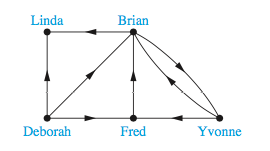
\includegraphics{acq} $$ \end{example} 

\begin{example} Influence Graphs: In studies of group behavior, it is observed that certain people can influence the thinking of others. A directed graph called an influence graph can be used to model this behavior. Each person of the group is represented by a vertex. There is a directed edge from vertex $a$ to vertex $b$ when the person represented by vertex $a$ can influence the person represented by vertex $b$. This graph does not contain loops and it does not contain multiple directed edges. In the group modeled by the influence graph below, Deborah cannot be influence but she can influence Brian, Fred and Linda. Also, Yvonne and Brian can influence each other. 
$$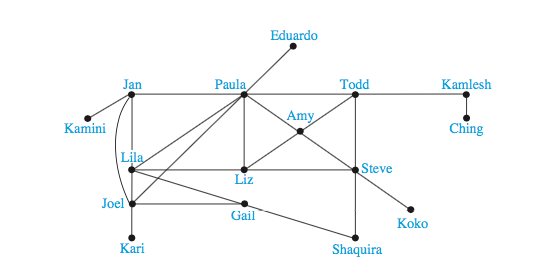
\includegraphics[scale = 0.65]{influence} $$ \end{example} 

\begin{example} Collaboration Graph: A collaboration graph is used to model social networks where two people are related by working together in a particular way. Collaboration graphs are simple graphs, as edges in these graphs are undirected and there are no multiple edges or loops. Vertices in these graphs represent people; two people are connected by an undirected edge when the people have collaborated. There are no loops nor multiple edges in these graphs. The Hollywood graph is a collaborator graph that represents actors by vertices and connects two actors with an edge if they have worked together on a movie or television show. The Hollywood graph is a huge graph with more than 1.5 million vertices. In an academic collaboration graph, vertices represent people (perhaps restricted to members of a certain academic community), and edges link two people if they have jointly published a paper. The collaboration graph for people who have published research papers in mathematics was found in 2004 to have more than 400,000 vertices and 675,000 edges and these numbers have grown considerably since then. Collaboration graphs have also been used in sports, where two professional athletes are considered to have collaborated if they have every played on the same team during a regular season of their sport. \end{example} 

\begin{example} Call Graphs: Graphs can be used to model telephone calls made in a network, such as a long distance telephone network. In particular, a directed multigraph can be used to model calls where each telephone number is represented by a vertex and each telephone call is represented by a directed edge. The edge representing a call starts at the telephone number from which the call was made and ends at the telephone number to which the call was made. Directed edges are needed because the direction in which the call is made matters. Multiple directed edges are needed because each particular telephone number can make several calls to a  second number. In the call graph below, seven telephone numbers are represented. The graph shows that three calls have been made from 732-555-1234 to 732-555-9876 and two in the other direction, but no calls have been made from 732-555-4444 to any of the other six numbers except 732-555-0011. When we care only whether there has been a call connecting two telephone numbers, we use an indirected graph with an edge connecting telephone numbers when there has been a call between these numbers, as represented in the second graph below. Call graphs that model actual calling activities can be huge. For example, one call graph studied at AT\&T, which models calls during 20 days, has about 290 million vertices and 4 billion edges. $$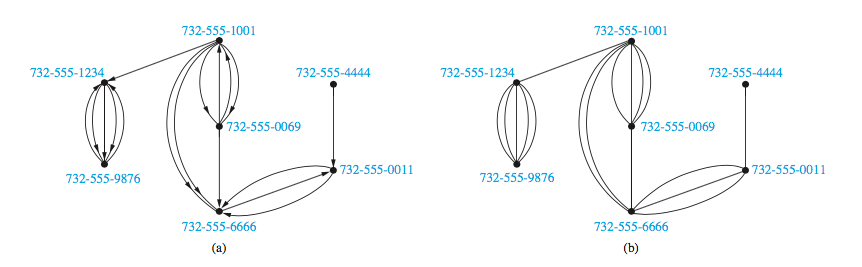
\includegraphics[scale = 0.5]{call} $$ \end{example} 

\begin{example} Web Graph: The World Wide Web can be modeled as a directed graph where each web page is represented by a vertex and where an edge starts at the web page $a$ and ends at the web page $b$ if there is a link on $a$ pointing to $b$. Because new web pages are created and others removed somewhere on the Web almost every second, the web graph changes on an almost continual basis. \end{example} 

\begin{example} Citation Graph: Graphs can be used to represent citations in different types of documents, including academic papers, patents, and legal opinions. In such graphs, each document is represented by a vertex, and there is an edge from one document to a second document if the first document cites the second document in its citation list. A citation graph is a directed graph without loops or multiple edges. \end{example} 

\begin{example} Module Dependency Graph: One of the most important tasks in designing software is how to structure a program into different parts, or modules. Understanding how the different modules of a program interact is essential not only for program design, but also for testing and maintenance of the resulting software. A module dependency graph provides a useful took for understanding how different modules of a program interact. In a program dependency graph, each module is represented by a vertex. There is a directed edge from a module to a second module if the second module depends on the first. An example of a program dependency graph for a web browser is shown below. $$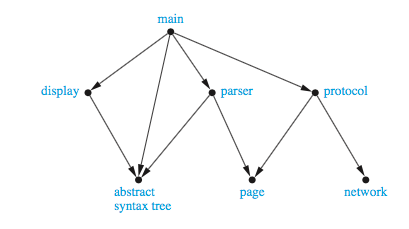
\includegraphics[scale = 0.4]{moduledependency}$$ \end{example} 

\begin{example} Precedence Graphs and Concurrent Processing: Computer programs can be executed more rapidly be executing certain statements concurrently. It is important not to execute a statement that requires results of statements not yet executed. The dependency of statements on previous statements can be represented by a directed graph. Each statement is represented by a vertex, and there is an edge from one statement to a second statement if the second statement cannot be executed before the first statement. This resulting graph is called a precedence graph. A computer program and its graph is shown below. For instance, the graph shows that statement $S_5$ cannot be executed before statements $S_1$, $S_2$ and $S_4$ are executed. 
$$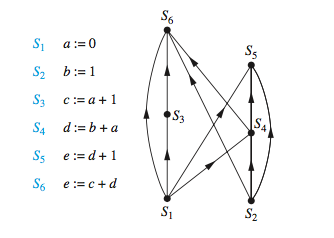
\includegraphics[scale = 0.5]{precedence}$$ \end{example} 

\begin{example} Airline Routes:Airline networks can be modeled by representing each airport by a vertex. In particular, model all the flights by a particular airline each day using a directed edge to represent each flight, going from the vertex representing the departure airport to the vertex representing the destination airport. The resulting graph will generally be a directed multigraph, as there may be multiple flights from one airport to some other airport during the same day. \end{example} 

\begin{example} Road Networks: Graphs can be used to model road networks. In such models, vertices represent intersections and edges represent roads. When all roads are two-way and there is at most one road connecting two intersections, use a simple undirected graph to model the road network. However, when roads are one-way and when there may be more than one road between two intersections, use undirected edges to represent the two way roads and directed edges to represent one way roads. Multiple undirected edges represent multiple two-way roads connecting the same two intersections. Multiple directed edges represent multiple one way roads that start at one intersection and end at a second intersection. Loops represent loop roads. Mixed graphs are needed to model road networks that include both one way and two way roads. \end{example} 

\begin{example} Niche Overlap Graphs in Ecology: Graphs are used in many models involving the interaction of different species of animals. For instance, the competition between species in an ecosystem can be modeled using a niche overlap graph. Each species is represented by a vertex. An undirected edge connects two vertices if the two species represented by these vertices compete. A niche overlap graph is a simple graph because no loops or multiple edges are needed in this model. The graph below models the ecosystem of a forest. It can be seen that squirrels and raccoons compete but that crows and shrews do not. $$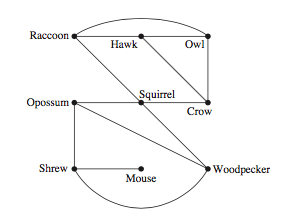
\includegraphics[scale = 0.7]{niche}$$ \end{example} 

\begin{example} Protein Interaction Graphs: A protein interaction in a living cell occurs when two or more proteins in that cell bind to perform a biological function. Because protein interactions are crucial for most biological features, many scientists work on discovering new proteins and understanding interactions between proteins. Protein interactions within a cell can be modeled using a protein interaction graph (or protein-protein interaction network), an undirected graph in which each protein is represented by a vertex, with an edge connecting the vertices representing each pair of proteins that interact. It is a challenging problem to determine genuine protein interactions in a cell, as experiments often produce false positives which conclude that two proteins interact when they really do not. Protein interaction graphs can be used to deduce important biological information, such as by identifying the most important proteins for various functions and the functionality of newly discovered proteins. Because there are thousands of different proteins in a typical cell, the protein interaction graph of a cell is extremely large and complex. For example, yeast cells have more than 6,000 proteins and more than 80,000 interactions between them are known. Human cells have more than 100,000 proteins with perhaps as many as 1,000,000 interactions between them. Additional vertices and edges are added to a protein interaction graph when new proteins and interactions between proteins are discovered. Because of the complexity of protein interaction graphs, they are often split into smaller graphs called modules that represent groups of proteins that are involved in a particular function of a cell. The graph below illustrates a module of the protein interaction graph described in [Bo04], comprising the complex of proteins that degrade RNA in human cells. 
$$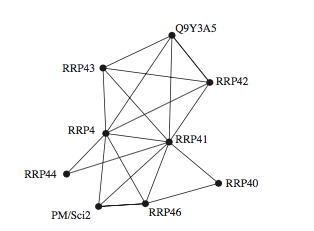
\includegraphics[scale = 0.6]{protein}$$ \end{example} 

\begin{example} Round-Robin Tournaments: A tournament where each team plays every other team exactly once and no ties are allowed is called a round-robin tournament. Such tournaments can be modeled using directed graphs where each team is represented by a vertex. Note that $(a, b)$ is an edge if team $a$ beats team $b$. This graph is a simple directed graph, containing no loops or multiple directed edges (because no two teams play each other more than once). Such a directed graph model is shown below. It is seen that Team 1 is undefeated in this tournament and Team 3 is winless. $$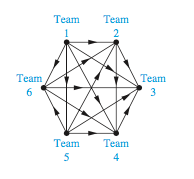
\includegraphics{roundrobin}$$ \end{example} 

\begin{example} Single-Elimination Tournaments: A tournament where each contestant is eliminated after one loss is called a single-elimination tournament. Single elimination tournaments are often used in sports, including tennis championships and the yearly NCAA basketball championship. This type of tournament can be modeled using a vertex to represent each game and directed edge to connect a game to the next game the winner of this game played in. The graph below represents the game played by the final 16 teams in the 2010 NCAA women's basketball tournament. $$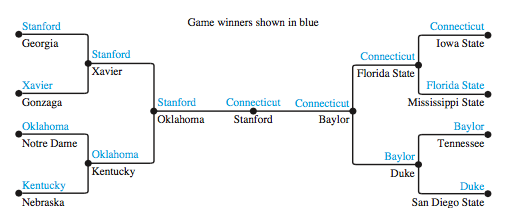
\includegraphics[width = \textwidth]{single}$$ \end{example} 

\subsection{Graph Terminology and Special Types of Graphs}
\begin{definition} Two vertices $u$ and $v$ in an undirected graph $G$ are called adjacent (or neighbors) in $G$ if $u$ and $v$ are endpoints of an edge $e$ of $G$. Such an edge $e$ is called incident with the vertices $u$ and $v$ and $e$ is said to connect $u$ and $v$. \end{definition} 
\begin{definition} The set of all neighbors of a vertex $v$ of $G = (V, E)$, denoted by $N(v)$ is called the neighborhood of $v$. If $A$ is a subset of $V$, demote $N(A)$ the set of all vertices in $G$ that are adjacent to at least one vertex in $A$. So, $N(A) = \bigcup_{v \in A} N(v) $. \end{definition} 
\begin{definition} The degree of a vertex in an undirected graph is the number of edges incident with it, except that a loop at a vertex contributes twice to the degree of that vertex. The degree of the vertex $v$ is denoted by deg($v$). \end{definition} 

\begin{definition} Isolated Vertex: a vertex of degree zero; not adjacent to any vertex \end{definition} 
\begin{definition} Pendant Vertex: a vertex of degree one; adjacent to exactly one other vertex \end{definition} 

\begin{theorem} Handshaking Theorem: Let $G = (V, E)$ be an undirected graph with $m$ edges. Then $$2n = \sum_{v \in V} \text{deg}(v)$$ This applies even if multiple edges and loops are present. \end{theorem} 

\begin{theorem} An undirected graph has an even number of vertices of odd degree. \end{theorem} 

\begin{definition} When $(u, v)$ is an edge of the graph $G$ with directed edges, $u$ is said to be adjacent to $v$ and $v$ is said to be adjacent to $u$. The vertex $u$ is called the initial vertex of $(u, v)$ and $v$ is called the terminal or end vertex of $(u, v)$. The initial vertex and terminal vertex of a loop are the same. \end{definition} 

\begin{definition} In a graph wth directed edges, the in-degree of a vertex $v$, denoted by deg$^{-1}(v)$, is the number of edges with $v$ as their terminal vertex. The out-degree of $v$, denoted by deg$^+(v)$, is the number of edges with $v$ as their initial vertex. Note that a loop at a vertex contributes 1 to both the in-degree and the out-degree of this vertex. \end{definition} 

\begin{theorem} Let $G = (V, E)$ be a graph with directed edges. Then $$\sum_{v \in V} \text{deg}^{-1}(v) = \sum_{v \in V} \text{deg}^+(v) = |E| $$ \end{theorem} 

\begin{definition} Underlying Undirected Graph: the undirected graph that results from ignoring directions of edges \end{definition} 
Note: A graph with directed edges and its underlying undirected graph have the same number of edges. 

\begin{definition} Complete Graph on $n$ Vertices ($K_n$): a simple graph that contains exactly one edge between each pair of distinct vertices $$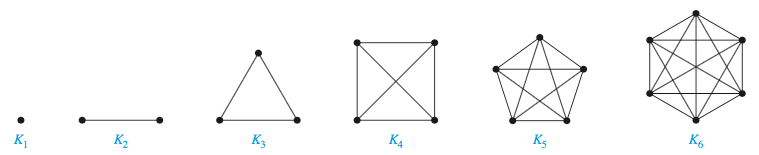
\includegraphics[width = \textwidth]{completegraphs}$$ \end{definition} 
\begin{definition} Noncomplete Graph: a simple graph for which there is at least one pair of distinct vertex not connected by an edge \end{definition} 

\begin{definition} Cycles ($C_n$): consists for $n$ ($n \geq 3$) vertices $v_1, v_2, \dots, v_n$ and edges $\{v_1, v_2\}, ~ \{v_2, v_3\}, \dots, \{v_{n - 1}, v_n\}$ and $\{v_n, v_1\}$ $$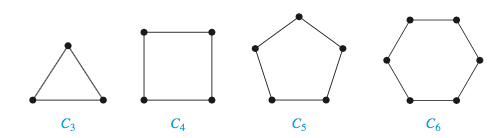
\includegraphics[width = \textwidth]{cycles} $$ \end{definition} 

\begin{definition} Wheels ($W_n$): obtained by adding an additional vertex to a cycle $C_n$, for $n n \geq 3$ and connected this new vertex to each of the $n$ vertices in $C_n$ by new edges $$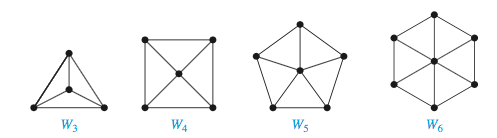
\includegraphics[width = \textwidth]{wheels}$$ \end{definition} 

\begin{definition} $n$-Dimensional Hypercube (or $n$-Cubes) ($Q_n$): a graph that has vertices representing the $2^n$ bit strings of length $n$. two vertices are adjacent if and only if the bit strings that they represent differ in exactly one bit position. \\ Note that a $(n + 1)$-cube $Q_{n + 1}$ can be constructed from the $n$-cube $Q_n$ by making two copies of $Q_n$, prefacing the labels on the vertices with a 0 in one copy of $Q_n$ and with a 1 in the other copy of $Q_n$ and adding edges connecting two vertices that have labels differing only in the first bit. $$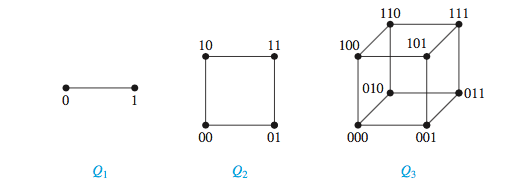
\includegraphics[width = \textwidth]{ncubes} $$\end{definition} 

\begin{definition} A simple graph $G$ is called bipartite if its vertex set $V$ can be partitioned into two disjoint sets $V_1$ and $V_2$ such that every edge in the graph connects a vertex in $V_1$ and a vertex in $V_2$ (so that no edge in $G$ connects exactly two vertices in $V_1$ or two vertices in $V_2$). When this condition holds, the pair ($V_1, V_2$) is called a bipartition of the vertex set $V$ of $G$. \end{definition} 

\begin{example} Is $C_6$ bipartite? \\ $C_6$ is bipartite because its vertex set can be partitioned into the two sets $V_1 = \{v_1, v_3, v_5\}$ and $V_2 = \{v_2, v_4, v_6\}$ and every edge of $C_6$ connects a vertex in $V_1$ and a vertex in $V_2$. $$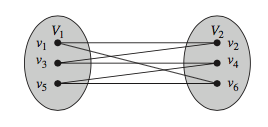
\includegraphics{c6bipartite}$$ \end{example} 

\begin{example} Is $K_3$ bipartite? \\ $K_3$ is not bipartite. Note that if the vertex set of $K_3$ was divided into two disjoint sets, one of the two sets must contain two vertices. If the graph were bipartite, these two vertices could not be connected by an edge, but in $K_3$ each vertex is connected to every other vertex by an edge. \end{example} 

\begin{example} Is the following graph bipartite? $$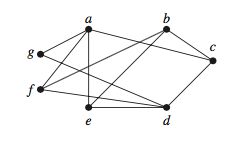
\includegraphics[scale = 0.7]{graphg}$$ This graph is bipartite because its vertex set is the union of two disjoint sets $\{a, b, d\}$ and $\{c, e, f, g\}$ and each edge connects a vertex in one of these subsets to a vertex in the other subset. Note that in order for the graph to be bipartite, it is not necessary that every vertex in $\{a, b, d\}$ be adjacent to every vertex in $\{c, e, f, g\}$. For instance, $b$ and $g$ are not adjacent. \end{example} 

\begin{example} Is the following graph bipartite? $$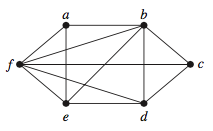
\includegraphics[scale = 0.7]{graphh}$$ This graph is not bipartite because its vertex set cannot be partitioned into two subsets so that edges do not connect two vertices from the same subset. \end{example} 

\begin{theorem} A simple graph is bipartite if and if it is possible to assign one of two different colors to each vertex of the graph so that no two adjacent vertices are assigned the same color. \end{theorem} 

\begin{definition} Complete Bipartite Graphs ($K_{m, n}$): a graph that has its vertex set partitioned into two subsets of $m$ and $n$ vertices, respectively with an edge between two vertices if and only if one vertex is in the first subset and the other vertex is in the second vertex $$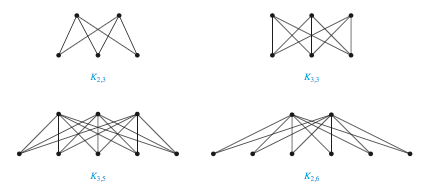
\includegraphics[scale = 0.7]{completebipartite} $$ \end{definition} 



\newpage
\subsection{Euler and Hamilton Paths}
\begin{definition} An Euler circuit in a graph $G$ is a simple circuit containing every edge of $G$. An Euler path in $G$ is a simple path containing every edge of $G$. \end{definition} 

\begin{example} Which of the undirected graphs have an Euler circuit? Of those that do not, which have an Euler path? $$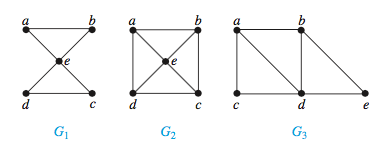
\includegraphics[scale = 0.7]{undirectedeuler}$$ 
The graph $G_1$ has an Euler circuit, for example, a, e, c, d, e, b, a. Neither of the graphs $G_2$ or $G_3$ has an Euler circuit. However, $G_3$ has an Euler path, namely, a, c, d, e, b, d, a, b. $G_2$ does not have an Euler path. \end{example} 

\begin{example} Which of the following directed graphs have an Euler circuit? Of those that do not, which have an Euler path? $$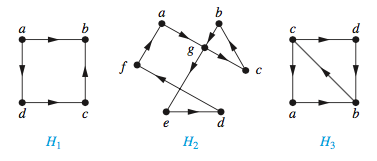
\includegraphics[scale = 0.7]{directedeuler}$$
The graph $H_2$ has an Euler circuit, for example, a, g, c, b, g, e, d, f, a. Neither $H_1$ nor $H_3$ has an Euler circuit. $H_3$ has an Euler path, namely, c, a, b, c, d, b, but $H_1$ does not. \end{example} 

\begin{theorem} A connected multigraph with at least two vertices has an Euler circuit if and only if each of its vertices has even degree. \end{theorem} 

\begin{theorem} A connected multigraph has an Euler path but not an Euler circuit if and only if it has exactly two vertices of odd degree. \end{theorem} 

\begin{alg} Constructing Euler Circuits \\ 
procedure $Euler$($G$: connected multigraph with all vertices of even degree)\\ 
$circuit$:= a circuit in $G$ beginning at an arbitrary chosen vertex with edges successively added to form a path that returns to this vertex \\
$H := G$ with the edges of this circuit removed \\
while $H$ has edges \\ 
\indent $subcircuit$:= a circuit in $H$ beginning at a vertex in $H$ that also is an endpoint of an edge of circuit \\
\indent $H:= H$ with edges of $subcircuit$ and all isolated vertices removed \\ 
\indent $circuit$ := $circuit$ with $subcircuit$ inserted at the appropriate vertex \\ 
return $circuit$ \{$circuit$ is an Euler circuit \} \end{alg} 

\begin{example} Which graphs have an Euler path? 
$$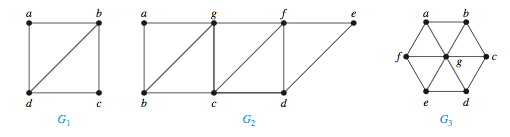
\includegraphics[width = \textwidth]{eulerpathex}$$ 
$G_1$ contains exactly two vertices of odd degree, namely, $b$ and $d$. Hence, it has an Euler path that must have $b$ and $d$ as its endpoints. One such Euler path is $d, a, b, c, d, b$. Similarly, $G_2$ has exactly two vertices of odd degree, namely, $b$ and $d$. So it has an Euler path that must have $b$ and $d$ as endpoints. One such Euler path is $b, a, g, f, e, d, c ,g, b, c, f, d$. $G_3$ has no Euler path because it has six vertices of odd degrees. \end{example} 

\begin{definition} A simple path in a graph $G$ that passes through every vertex exactly once is called a Hamilton path, and a simple circuit in a graph $G$ that passes through every vertex exactly once is called a Hamilton circuit. That is, the simplest path $x_0, x_1, \dots, x_{n - 1}, x_n$ in the graph $G = (V, E)$ is a Hamilton path if $V = \{x_0, x_1, \dots, x_{n - 1}, x_n\}$ and $x_i \neq x_j$ for $0 \leq i < j \leq n$ and the simplest circuit $x_0, x_1, \dots, x_{n - 1}, x_n, x_0$ (with $n > 0$) is a Hamilton circuit if $x_0, x_1, \dots, x_{n - 1}, x_n$ is a Hamilton path. \end{definition} 

\begin{example} Which of the simple graphs below have a Hamilton circuit or, if not, a Hamilton path? 
$$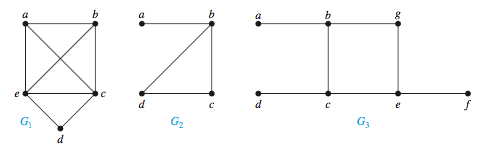
\includegraphics[width = \textwidth]{hamiltonex}$$ 
$G_1$ has a Hamilton circuit: $a, b, c, d, e, a$. There is no Hamilton circuit in $G_2$ (this can be seen by noting that any circuit containing every vertex must contain the edge $\{a, b\}$ twice), but $G_2$ does have a Hamilton path, namely, $a, b, c, d$. $G_3$ has neither a Hamilton circuit nor a Hamilton path, because any path containing all vertices must contain one of the edges $\{a, b\}$, $\{e, f\}$ and $\{c, d\}$ more than once. \end{example} 

\begin{example} Show that neither of the graphs below has a Hamilton circuit. 
$$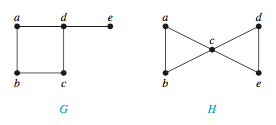
\includegraphics[width = \textwidth]{hamiltonnot} $$ 
There is no Hamilton circuit in $G$ because $G$ has a vertex of degree one, namely, $e$. In the case of $H$, because the degrees of the vertices $a, b, d$, and $e$ are all two, every edge incident with these vertices must be part of any Hamilton circuit. It is now easy to see that no Hamilton circuit can exist in $H$, for any Hamilton circuit would have to contain four edges incident with $c$, which is impossible. \end{example} 

\begin{example} Show that $K_n$ has a Hamilton circuit whenever $n \geq 3$. \\
A Hamilton circuit in $K_n$ can be formed beginning at any vertex. Such a circuit can be built by visiting vertices any order, as long as the path begins and ends at the same vertex and visits each other vertex exactly once. This is possible because there are edges in $K_n$ between any two vertices. \end{example} 

\begin{theorem} Dirac's Theorem: If $G$ is a simple graph with $n$ vertices with $n \geq 3$ such that the degree of every vertex in $G$ is at least $\frac{n}{2}$, then $G$ has a Hamilton circuit. \end{theorem} 

\begin{theorem} Ore's Theorem: If $G$ is a simple graph with $n$ vertices with $n \geq 3$ such that deg($u$) + deg($v$) $\geq n$ for every pair of nonadjacent vertices $u$ and $v$ in $G$, then $G$ has a Hamilton circuit. \end{theorem} 

\subsection{Shortest-Path Problems}

\begin{definition} Weighed Graphs: graphs that have a number assigned to each edge \end{definition}

\begin{definition} The length of a path in a weighed graph is the sum of the weights of the edges of this path. \end{definition} 

\begin{example} What is the length of a shortest path between $a$ and $z$ in the weighed graph below? \
$$ 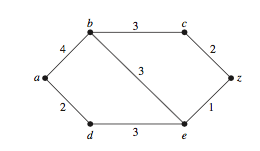
\includegraphics[width = \textwidth]{weighedgraph}$$ 
The only paths starting at $a$ that contain no vertex other than $a$ are formed by adding an edge that has $a$ as one endpoint. These paths have only one edge. There are $a, b$ of length 4 and $a, d$ of length 2. It follows that $d$ is the closest vertex to $a$, and the shortest path from $a$ to $d$ has length 2. To find the second closest vertex, examine all paths that begin with the shortest path from $a$ to a vertex in the set $\{a, d\}$, followed by an edge that has one endpoint in $\{a, d\}$ and its other endpoint not in this set. There are two such paths to consider, $a, d, e$ of length 7 and $a, b$ of length 4. Hence, the second closest vertex to $a$ is $b$ and the shortest path from $a$ to $b$ has length 4. To find the third closest vertex to $a$, examine only the paths that begin with the shortest path from $a$ to a vertex in the set $\{a, d, b\}$, followed by an edge that has one endpoint in the set $\{a, d, b\}$ and its other endpoint not in this set. There are three such paths, $a, b, c$ of length 7, $a, b, e$ of length 7 and $a, d, e$ of length 5. Because the shortest of these paths is $a, d, e$, the third closest vertex to $a$ is $e$ and the length of the shortest path from $a$ to $e$ is 5. To find the fourth closest vertex to $a$, examine only the paths that begin with the shortest path from $a$ to a vertex in the set $\{a, d, b, e\}$ followed by an edge that has one endpoint in the set $\{a, d, b, e\}$ and its other endpoint not in this set. There are two such paths, $a, b, c$ of length 7 and $a, d, e, z$ of length 6. Because the shorter of these paths is $a, d, e, z$, the fourth closest vertex to $a$ is $z$ and the length of the shortest path from $a$ to $z$ is 6. \end{example}  \newpage

\begin{alg} Dijkstra's Algorithm for Finding the Length of the Shortest Path \\ 

Dijkstra's algorithm proceeds by finding the length of a shortest path from $a$ to a first vertex, the length of a shortest path from $a$ to a second vertex, and so on, until the length of a shortest path from $a$ to $z$ is found. As a side benefit, this algorithm is easily extended to find the length of the shortest path from $a$ to all other vertices of the graph, and not just to $z$.\\ The algorithm relies on a series of iterations. A distinguished set of vertices is constructed by adding one vertex at each iteration. A labeling procedure is carried out at each iteration. In this labeling procedure, a vertex $w$ is labeled with the length of a shortest path from a to w that contains only vertices already in the distinguished set. The vertex added to the distinguished set is one with a minimal label among those vertices not already in the set.
We now give the details of Dijkstra?s algorithm. It begins by labeling $a$ with 0 and the other vertices with $\infty$. We use the notation $L_0(a) = 0$ and $L_0(v) = \infty$ for these labels before any iterations have taken place (the subscript 0 stands for the ``0th'' iteration). These labels are the lengths of shortest paths from $a$ to the vertices, where the paths contain only the vertex $a$. (Because no path from $a$ to a vertex different from $a$ exists, $\infty$ is the length of a shortest path between $a$ and this vertex.) \\
Dijkstra?s algorithm proceeds by forming a distinguished set of vertices. Let $S_k$ denote this set after $k$ iterations of the labeling procedure. Begin with $S_0 = \emptyset$. The set $S_k$ is formed from $S_{k-1}$ by adding a vertex $u$ not in $S_{k-1}$ with the smallest label.\\
Once $u$ is added to $S_k$, update the labels of all vertices not in $S_k$, so that $L_k(v)$, the label of the vertex $v$ at the $k$th stage, is the length of a shortest path from $a$ to $v$ that contains vertices only in $S_k$ (that is, vertices that were already in the distinguished set together with $u$). Note that the way we choose the vertex $u$ to add to $S_k$ at each step is an optimal choice at each step, making this a greedy algorithm. \\
Let $v$ be a vertex not in $S_k$. To update the label of $v$, note that $L_k (v)$ is the length of a shortest path from $a$ to $v$ containing only vertices in $S_k$. The updating can be carried out efficiently when this observation is used: A shortest path from $a$ to $v$ containing only elements of $S_k$ is either a shortest path from $a$ to $v$ that contains only elements of $S_{k-1}$ (that is, the distinguished vertices not including $u$), or it is a shortest path from $a$ to $u$ at the $(k - 1)$st stage with the edge $\{u, v\}$ added. In other words,
$$ L_k(a, v) = \min\{L_{k-1}(a, v), L_{k-1}(a, u) + w(u, v)\}$$ 
where $w(u, v)$ is the length of the edge with $u$ and $v$ as endpoints. This procedure is iterated by successively adding vertices to the distinguished set until $z$ is added. When $z$ is added to the distinguished set, its label is the length of a shortest path from $a$ to $z$. \end{alg}

\begin{alg} Dijkstra's Algorithm \\ 
procedure $Dijkstra$($G$: weighed connected simple graph, with all weights positive) \\ 
\{$G$ has vertices $a = v_0, v_1, \dots, v_n = z$ and lengths $w(v_i, v_j)$ where $w(v_i, v_j) = \infty$ if $\{v_i, v_j\}$ is not an edge in $G$\} \\
for $i := 1$ to $n$ \\ 
\indent $L(v_i) := \infty $
$L(a) := 0$ \\ 
$S := \emptyset$ \\ 
\{the labels are now initialized so that the label of $a$ is 0 and all other labels are $\infty$ and $S$ is the empty set \} \\
while $z \notin S$ \\
\indent $u$:= a vertex not in $S$ with $L(u)$ minimal \\ 
\indent $S := S \bigcup \{u\}$ \\
\indent for all vertices $v$ not in $S$ \\
\indent \indent if $L(u) + w(u, v) < L(v)$ then $L(v) := L(u) + w(u, v)$ \\ 
\indent \indent \{this adds a vertex to $S$ with minimal label and updates the labels of vertices not in $S$\} \\
return $L(z)$ \{$L(z)$ = length of a shortest path from $a$ to $z$\} \end{alg} 

\begin{example} Use Dijkstra's algorithm to find the length of a shortest path between the vertices $a$ and $z$ in the weighed graph below. 
$$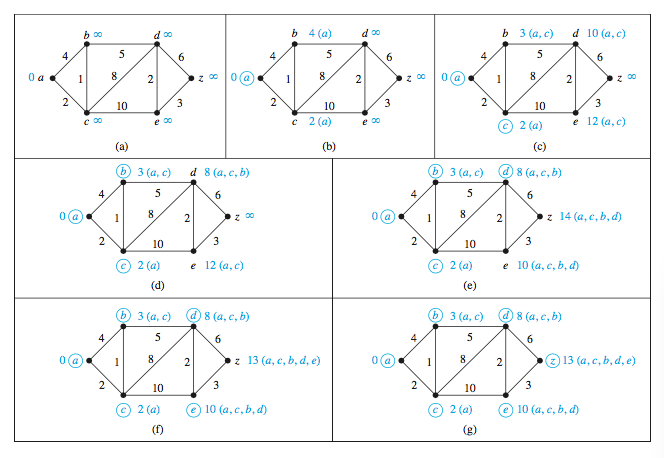
\includegraphics[width = \textwidth]{dijkstra}$$ \end{example} 

\begin{theorem} Dijkstra's algorithm finds the length of a shortest path between two vertices in a connected simple undirected weighted graph. \end{theorem} 

\begin{theorem} Dijkstra's algorithm uses $O(n^2)$ operations (additions and comparisons) to find the length of a shortest path between two vertices in a connected simple undirected weighted graph with $n$ vertices. \end{theorem} 


























\end{document}